% !TeX root = ../../progress-sem1.tex
% 3.x การพัฒนาระบบ: work done in semester 1 (M0-M3)
\section{การพัฒนาระบบ}
\thaijustify{
  ในภาคการศึกษาที่ 1 การพัฒนาระบบดำเนินการตาม milestone M0 ถึง M3 โดยใช้ GitHub เป็นที่เก็บซอร์สโค้ด ทุกการเปลี่ยนแปลงผ่าน pull request และตั้งชื่อตามรูปแบบ conventional commit จนถึงวันที่ 26 พฤศจิกายน 2569 มีการ commit ทั้งหมด 178 ครั้ง รายละเอียดของแต่ละ milestone มีดังนี้
}

\subsection{M0: Foundation}
\thaijustify{
  ช่วง Foundation เป็นการวางโครงสร้างพื้นฐานของโปรเจกต์ ได้แก่
  \begin{itemize}
    \item \textbf{โครงสร้างซอร์สโค้ด}\\
      monorepo ที่มี frontend และ backend ใช้คำสั่งเดียวในการรัน build, lint และ test ทั้งระบบ
    \item \textbf{สภาพแวดล้อมสำหรับพัฒนา}\\
      ใช้ Docker Compose รัน PostgreSQL และ Redis มีสคริปต์สร้างไฟล์ตั้งค่า สร้างผู้ใช้ทดสอบ และออก token สำหรับทดสอบ API โดยไม่ต้องเข้าสู่ระบบผ่าน Google
    \item \textbf{Data model}\\
      ออกแบบ schema ของฐานข้อมูลครอบคลุมทุก milestone ตั้งแต่ผู้ใช้จนถึงรายงาน (หัวข้อ~\ref{sec:er-diagram}) และจัดการการเปลี่ยนแปลงด้วย migration ซึ่งมีทั้งหมด 7 ชุด โดยกำหนดให้ migration ที่ merge แล้วแก้ไขไม่ได้ เพื่อให้ฐานข้อมูลของทุกคนตรงกัน
    \item \textbf{Design system}\\
      ใช้ shadcn/ui เป็นพื้นฐานของหน้าจอแพลตฟอร์ม และเตรียม UI kit สองชุด คือ shadcn/ui และ MUI ให้ AI ใช้สร้างหน้าจอตามที่นักออกแบบเลือก
    \item \textbf{PDPA}\\
      ออกแบบการเก็บความยินยอมของผู้เข้าร่วมทดสอบพร้อมเวอร์ชันของข้อความ เพื่อใช้ใน M4
    \item \textbf{CI}\\
      GitHub Actions ตรวจทุก pull request โดยเรียงเป็นสามขั้น คือ ชื่อ pull request, lint และ build
  \end{itemize}
  ส่วนที่ยังไม่ได้ทำคือการ deploy อัตโนมัติ (CD) และระบบเก็บ event analytics
}

\subsection{M1: Secure Access}
\thaijustify{
  ระบบยืนยันตัวตนปัจจุบันใช้การเข้าสู่ระบบด้วยบัญชี Google ผ่าน OAuth 2.0 เมื่อเข้าสู่ระบบสำเร็จ backend ออก access token แบบ JWT ที่มีอายุ 15 นาที และ refresh token ที่มีอายุ 30 วัน refresh token ถูกเก็บเป็นค่า hash และเปลี่ยนใหม่ทุกครั้งที่ใช้ (token rotation) หากมีการนำ token ที่ถูกใช้ไปแล้วกลับมาใช้ซ้ำ ระบบจะถือว่า token รั่วไหลและยกเลิก token ทั้งกลุ่มของการเข้าสู่ระบบนั้น
}
\thaijustify{
  การควบคุมสิทธิ์ใช้แนวทาง permission-based access control กล่าวคือ แต่ละบทบาทในโปรเจกต์ (Designer, Project Manager, Client และ Developer) ได้รับชุดสิทธิ์ เช่น \texttt{design:write}, \texttt{design:approve} และ \texttt{handoff:read} และ API แต่ละเส้นตรวจเฉพาะสิทธิ์ที่ต้องใช้ ไม่ได้ตรวจชื่อบทบาทโดยตรง ทำให้ปรับสิทธิ์ของแต่ละบทบาทได้ในที่เดียว นอกจากนี้ระบบบันทึกการกระทำสำคัญลง audit log และมี end-to-end test ตรวจการควบคุมสิทธิ์
}
\thaijustify{
  หน้าจอสมัครสมาชิก เข้าสู่ระบบ และลืมรหัสผ่านพัฒนาส่วน frontend แล้ว ส่วนการสมัครด้วยอีเมลและรหัสผ่าน การยืนยันอีเมล และการรีเซ็ตรหัสผ่านฝั่ง backend อยู่ระหว่างพัฒนาใน branch แยก และจะรวมเข้า branch หลักภายในภาคการศึกษาที่ 1
}
\begin{figure}[H]
  \centering
  \subfloat[เข้าสู่ระบบ]{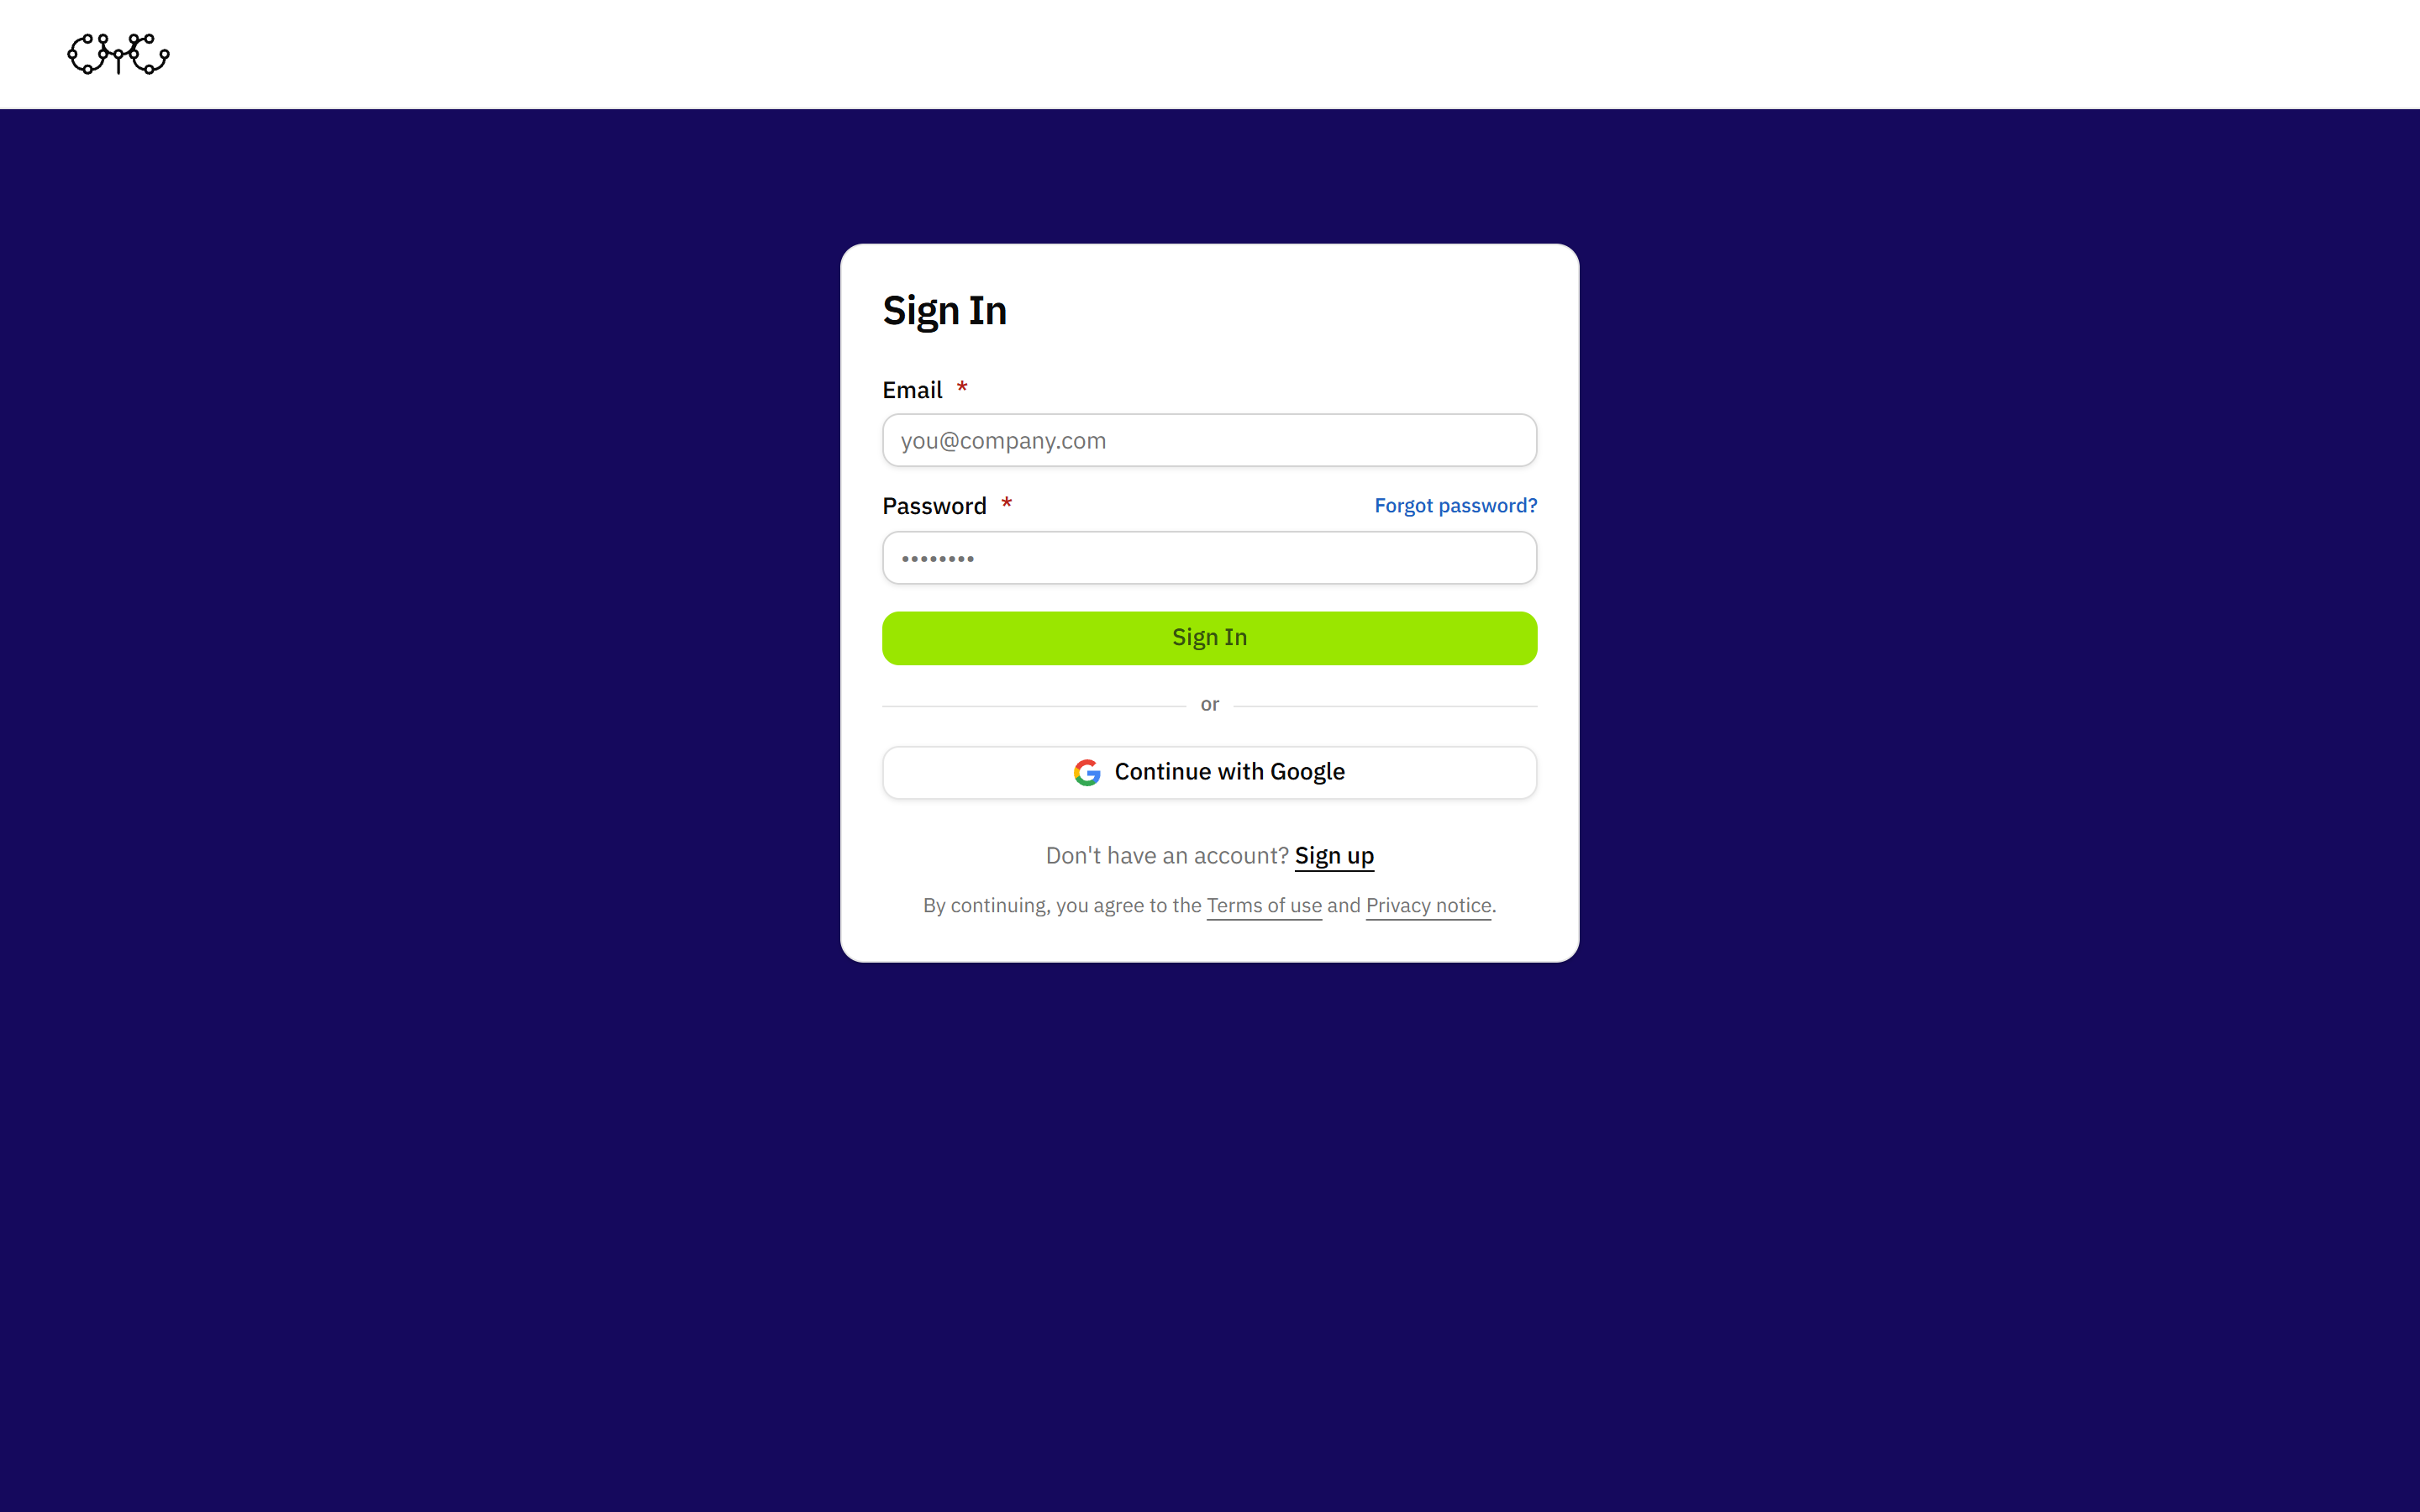
\includegraphics[width=0.49\linewidth]{figures/ch3-methodology/screens/signin.png}}\hfill
  \subfloat[สมัครสมาชิก]{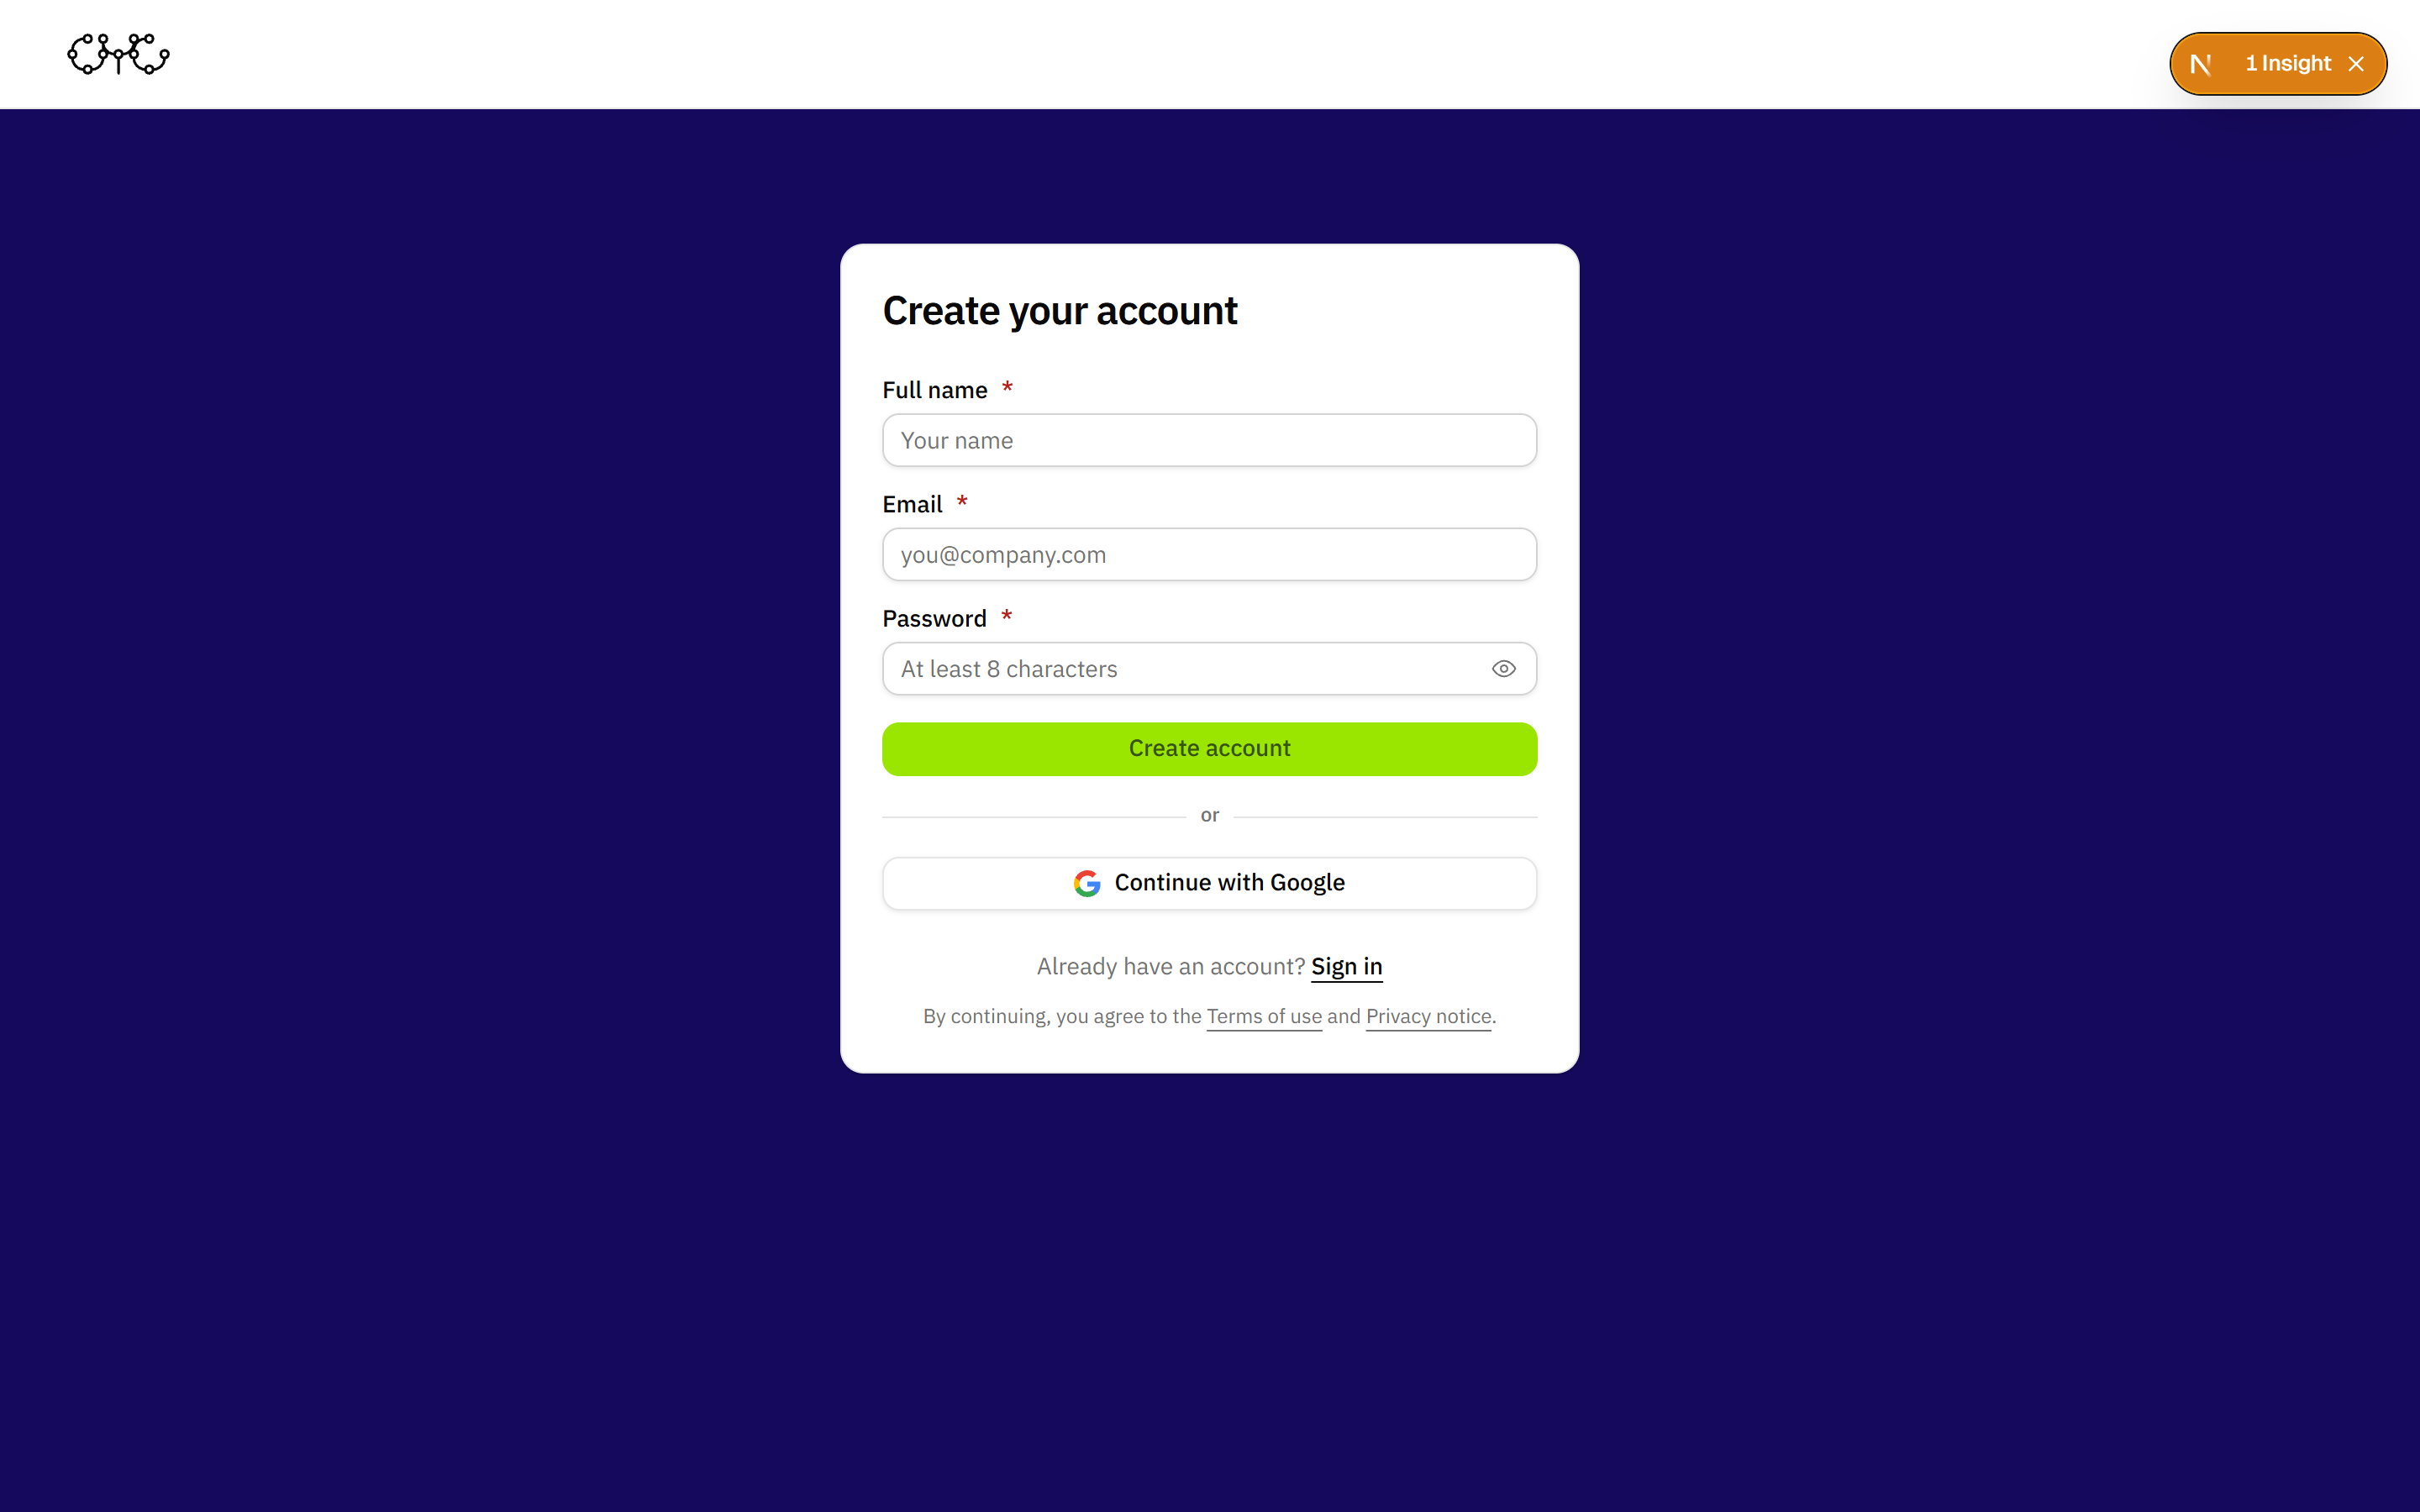
\includegraphics[width=0.49\linewidth]{figures/ch3-methodology/screens/signup.png}}
  \caption{หน้าจอเข้าสู่ระบบและสมัครสมาชิก}
  \label{fig:screen-auth}
\end{figure}

\subsection{M2: Project Setup}
\thaijustify{
  ผู้ใช้สร้าง workspace ตั้งรูปประจำ workspace และเชิญสมาชิกด้วยอีเมลได้ ภายใน workspace นักออกแบบสร้างโปรเจกต์ กำหนดสมาชิกและบทบาทในโปรเจกต์ และค้นหาหรือกรองโปรเจกต์ได้ทั้งแบบรายการและแบบแกลเลอรี
}
\thaijustify{
  ความต้องการทางการออกแบบ (design intent) ของโปรเจกต์ประกอบด้วยเป้าหมายของการออกแบบ design system ที่เลือก (shadcn/ui หรือ MUI) มาตรฐานการเข้าถึง (ค่าเริ่มต้น WCAG 2.1 AA) แนวทางการออกแบบ สีแบรนด์สามสี แนวทาง CI และ tone of voice ทุกครั้งที่แก้ไข ระบบจะเพิ่มเลขเวอร์ชันของ design intent และงานสร้าง UI แต่ละครั้งเก็บสำเนาของ design intent ที่ใช้ไว้ ทำให้ design intent เป็น context ที่ AI นำไปใช้ซ้ำได้ และตรวจสอบย้อนหลังได้ว่า UI แต่ละชุดสร้างจาก design intent ฉบับใด นอกจากนี้นักออกแบบเพิ่ม persona ของผู้ใช้เป้าหมายเองได้ และหน้าภาพรวมของโปรเจกต์แสดงกิจกรรมล่าสุดจาก audit log
}
\begin{figure}[H]
  \centering
  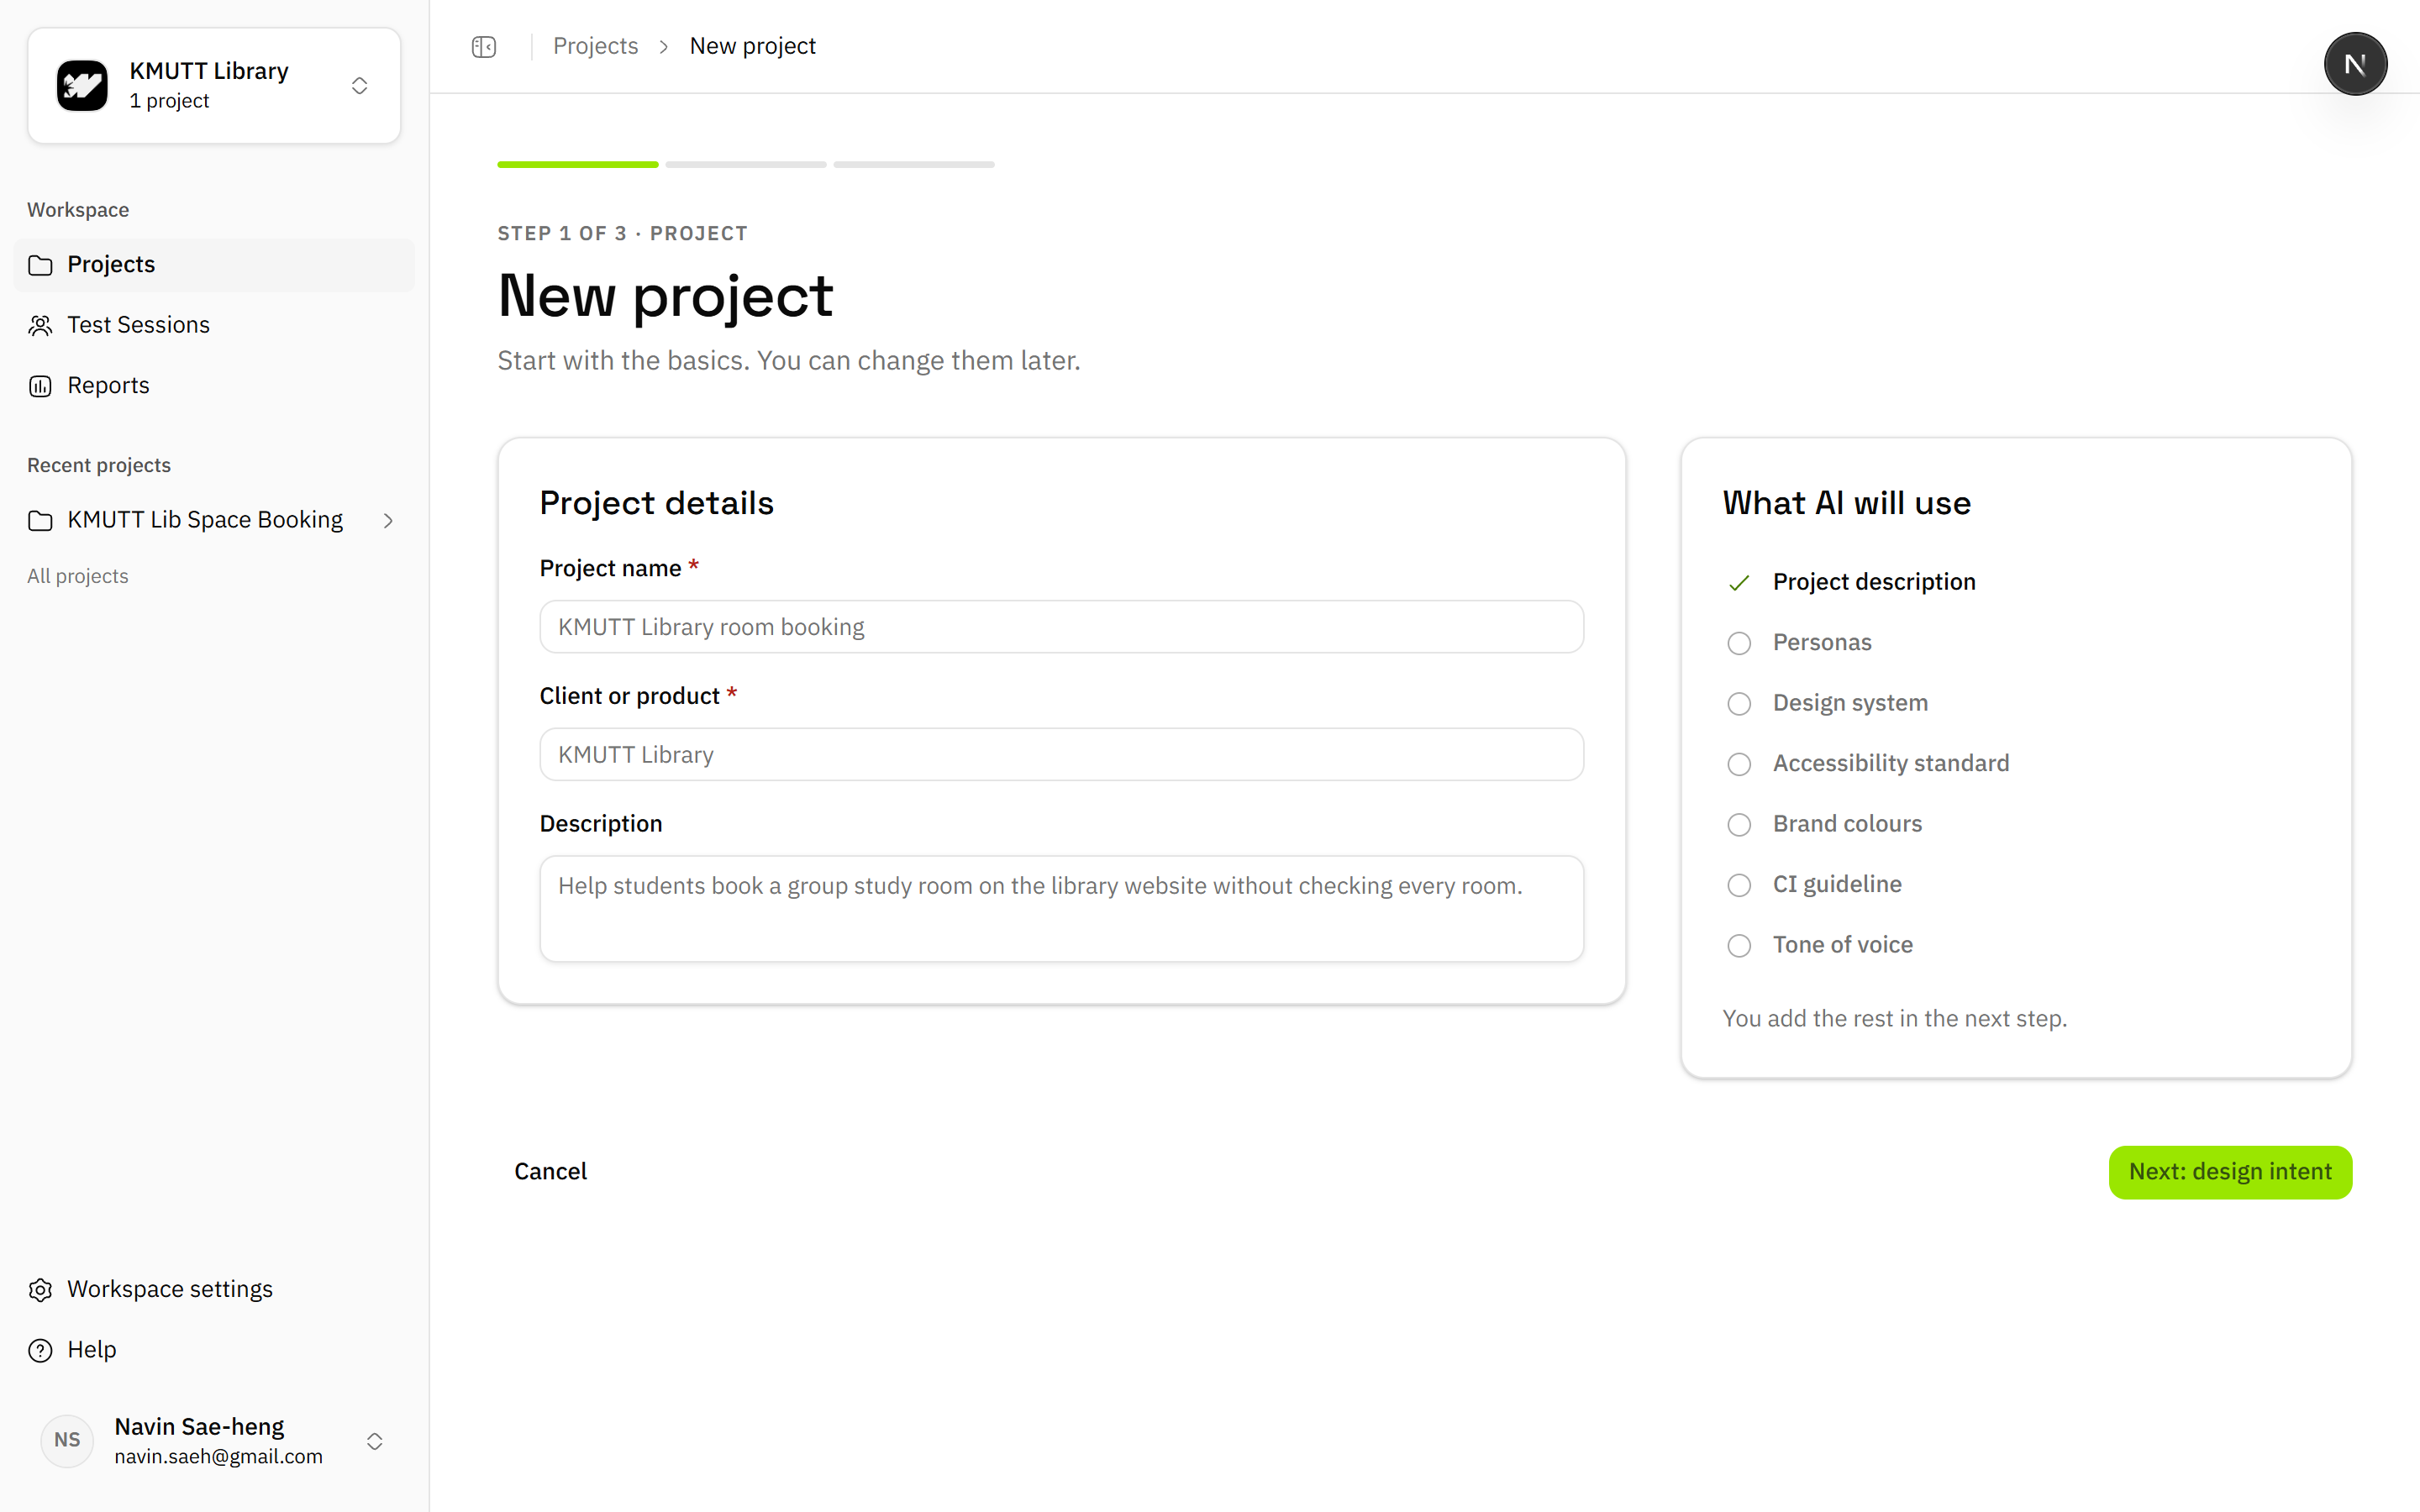
\includegraphics[width=0.9\linewidth]{figures/ch3-methodology/screens/project-new.png}
  \caption{หน้าจอสร้างโปรเจกต์ (ขั้นที่ 1 จาก 3 ของ wizard)}
  \label{fig:screen-project-new}
\end{figure}
\begin{figure}[H]
  \centering
  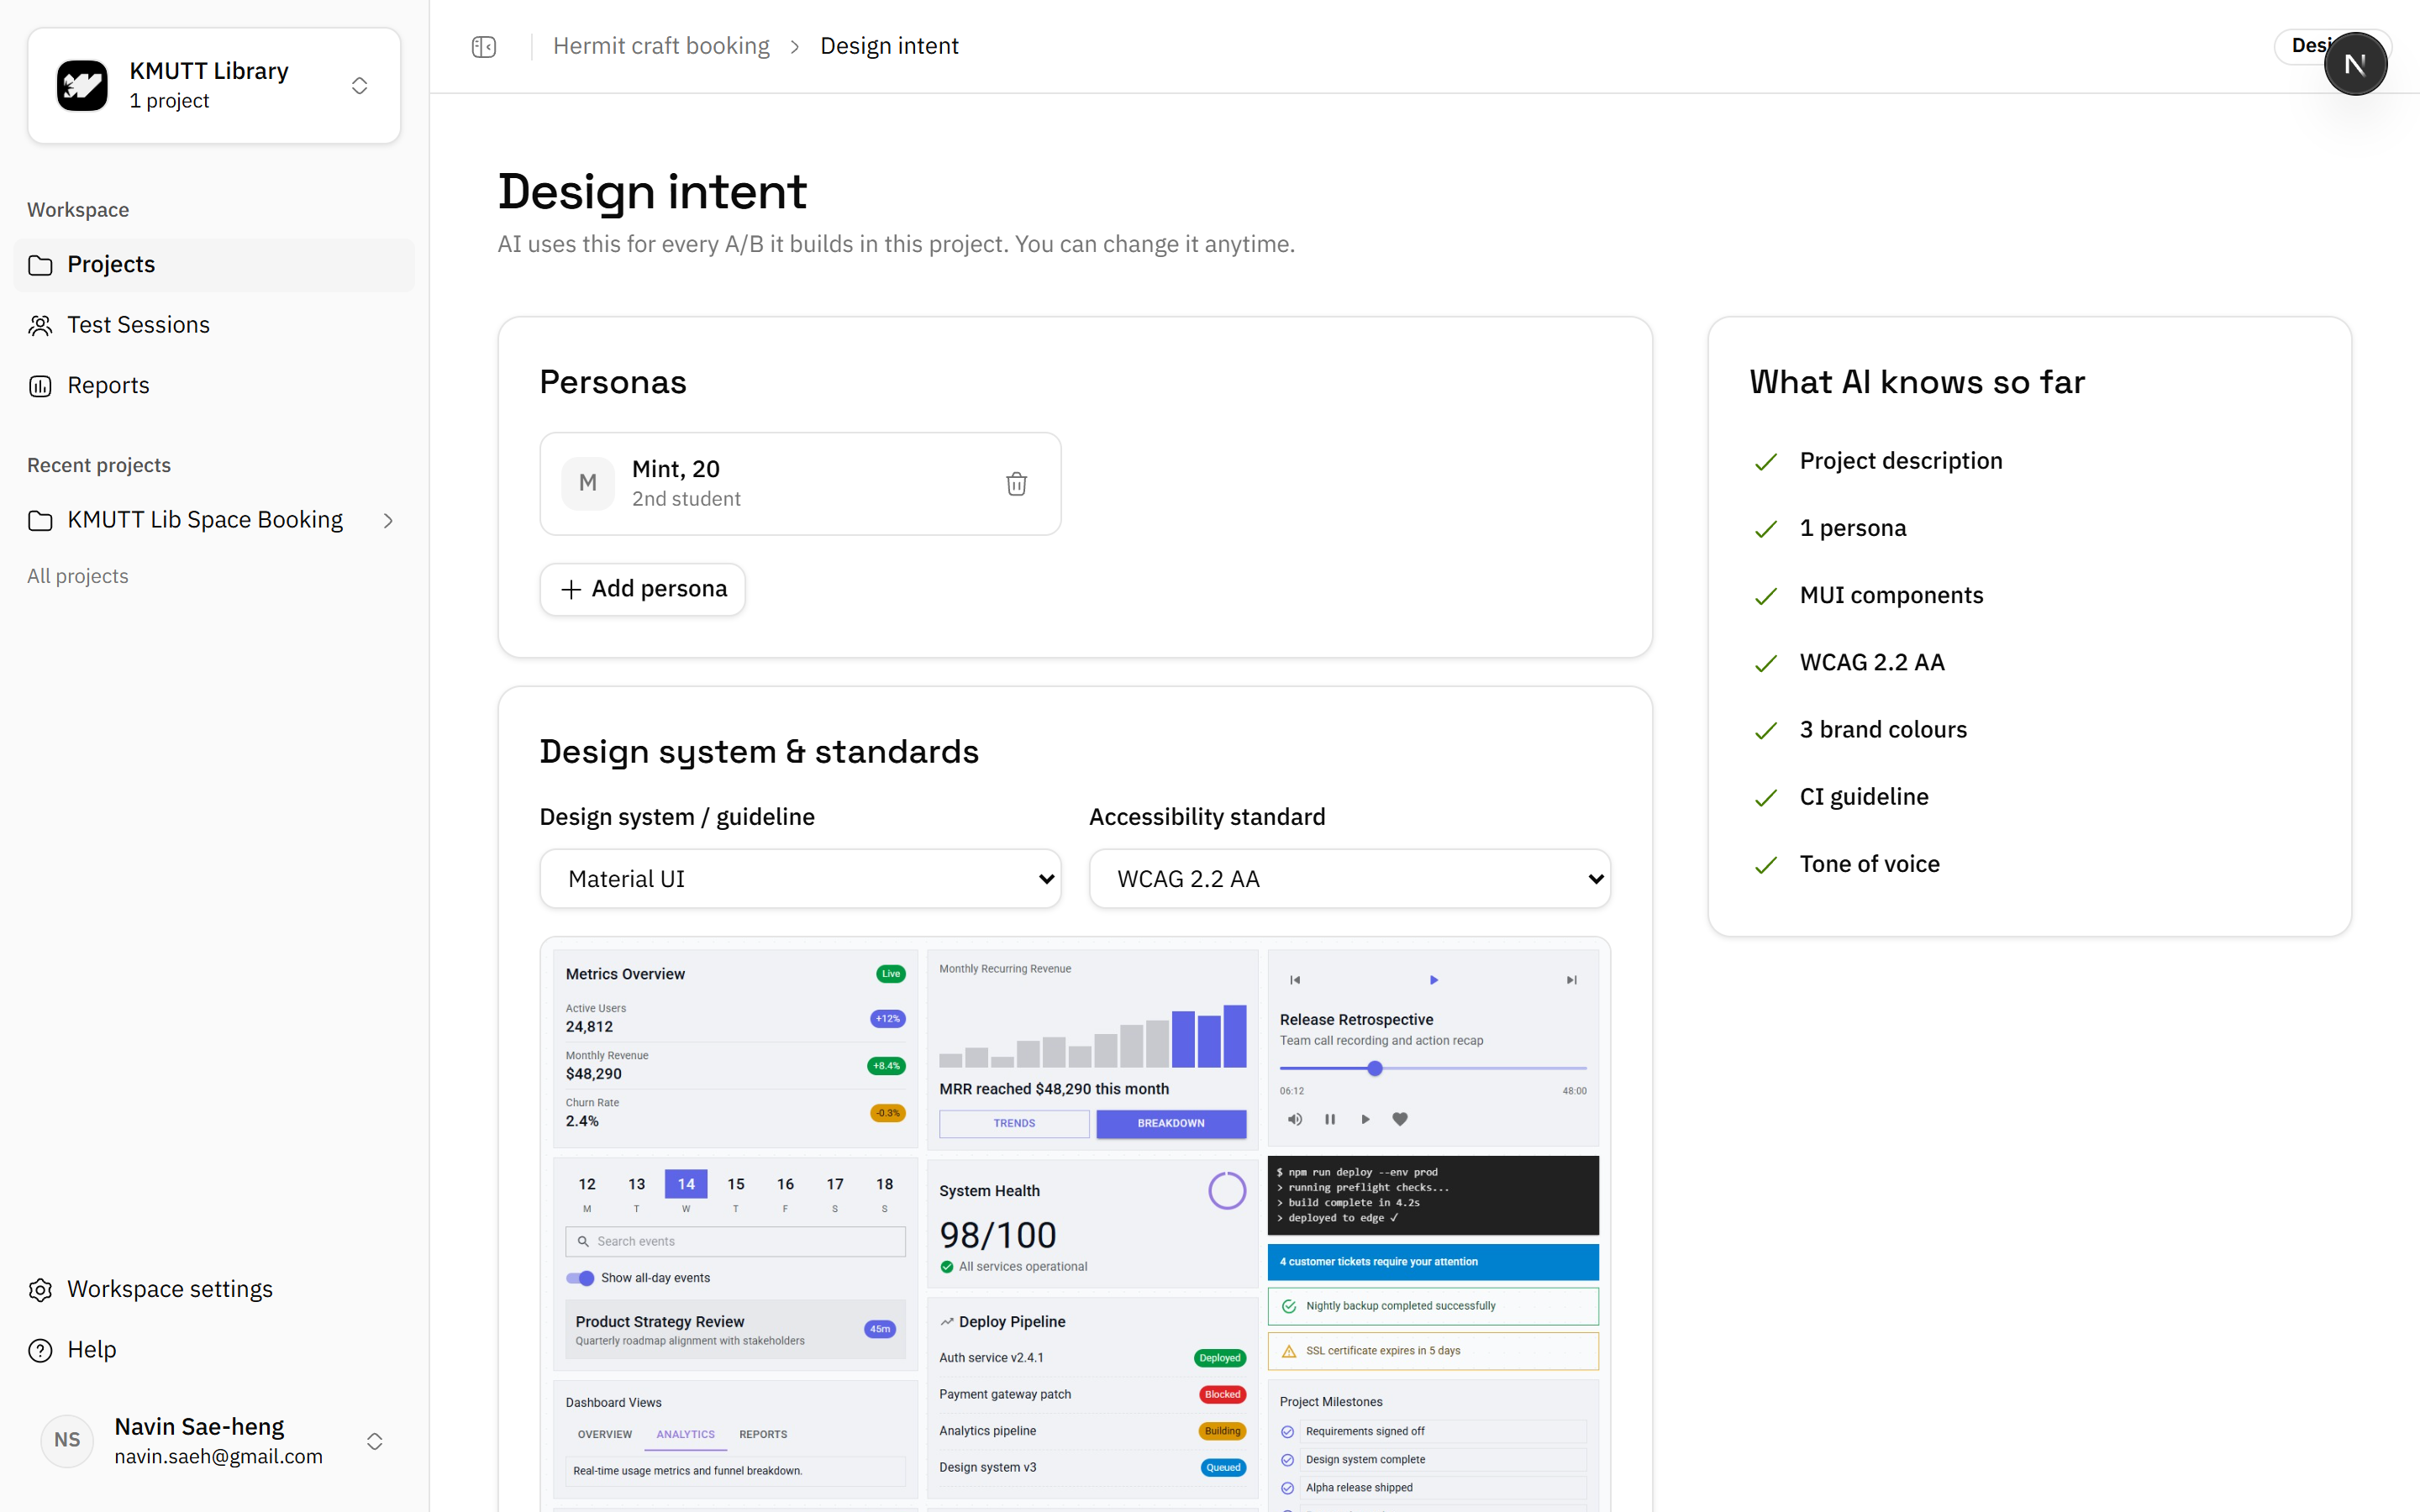
\includegraphics[width=0.9\linewidth]{figures/ch3-methodology/screens/design-intent.png}
  \caption{หน้าจอกำหนดความต้องการทางการออกแบบ (design intent)}
  \label{fig:screen-design-intent}
\end{figure}
\begin{figure}[H]
  \centering
  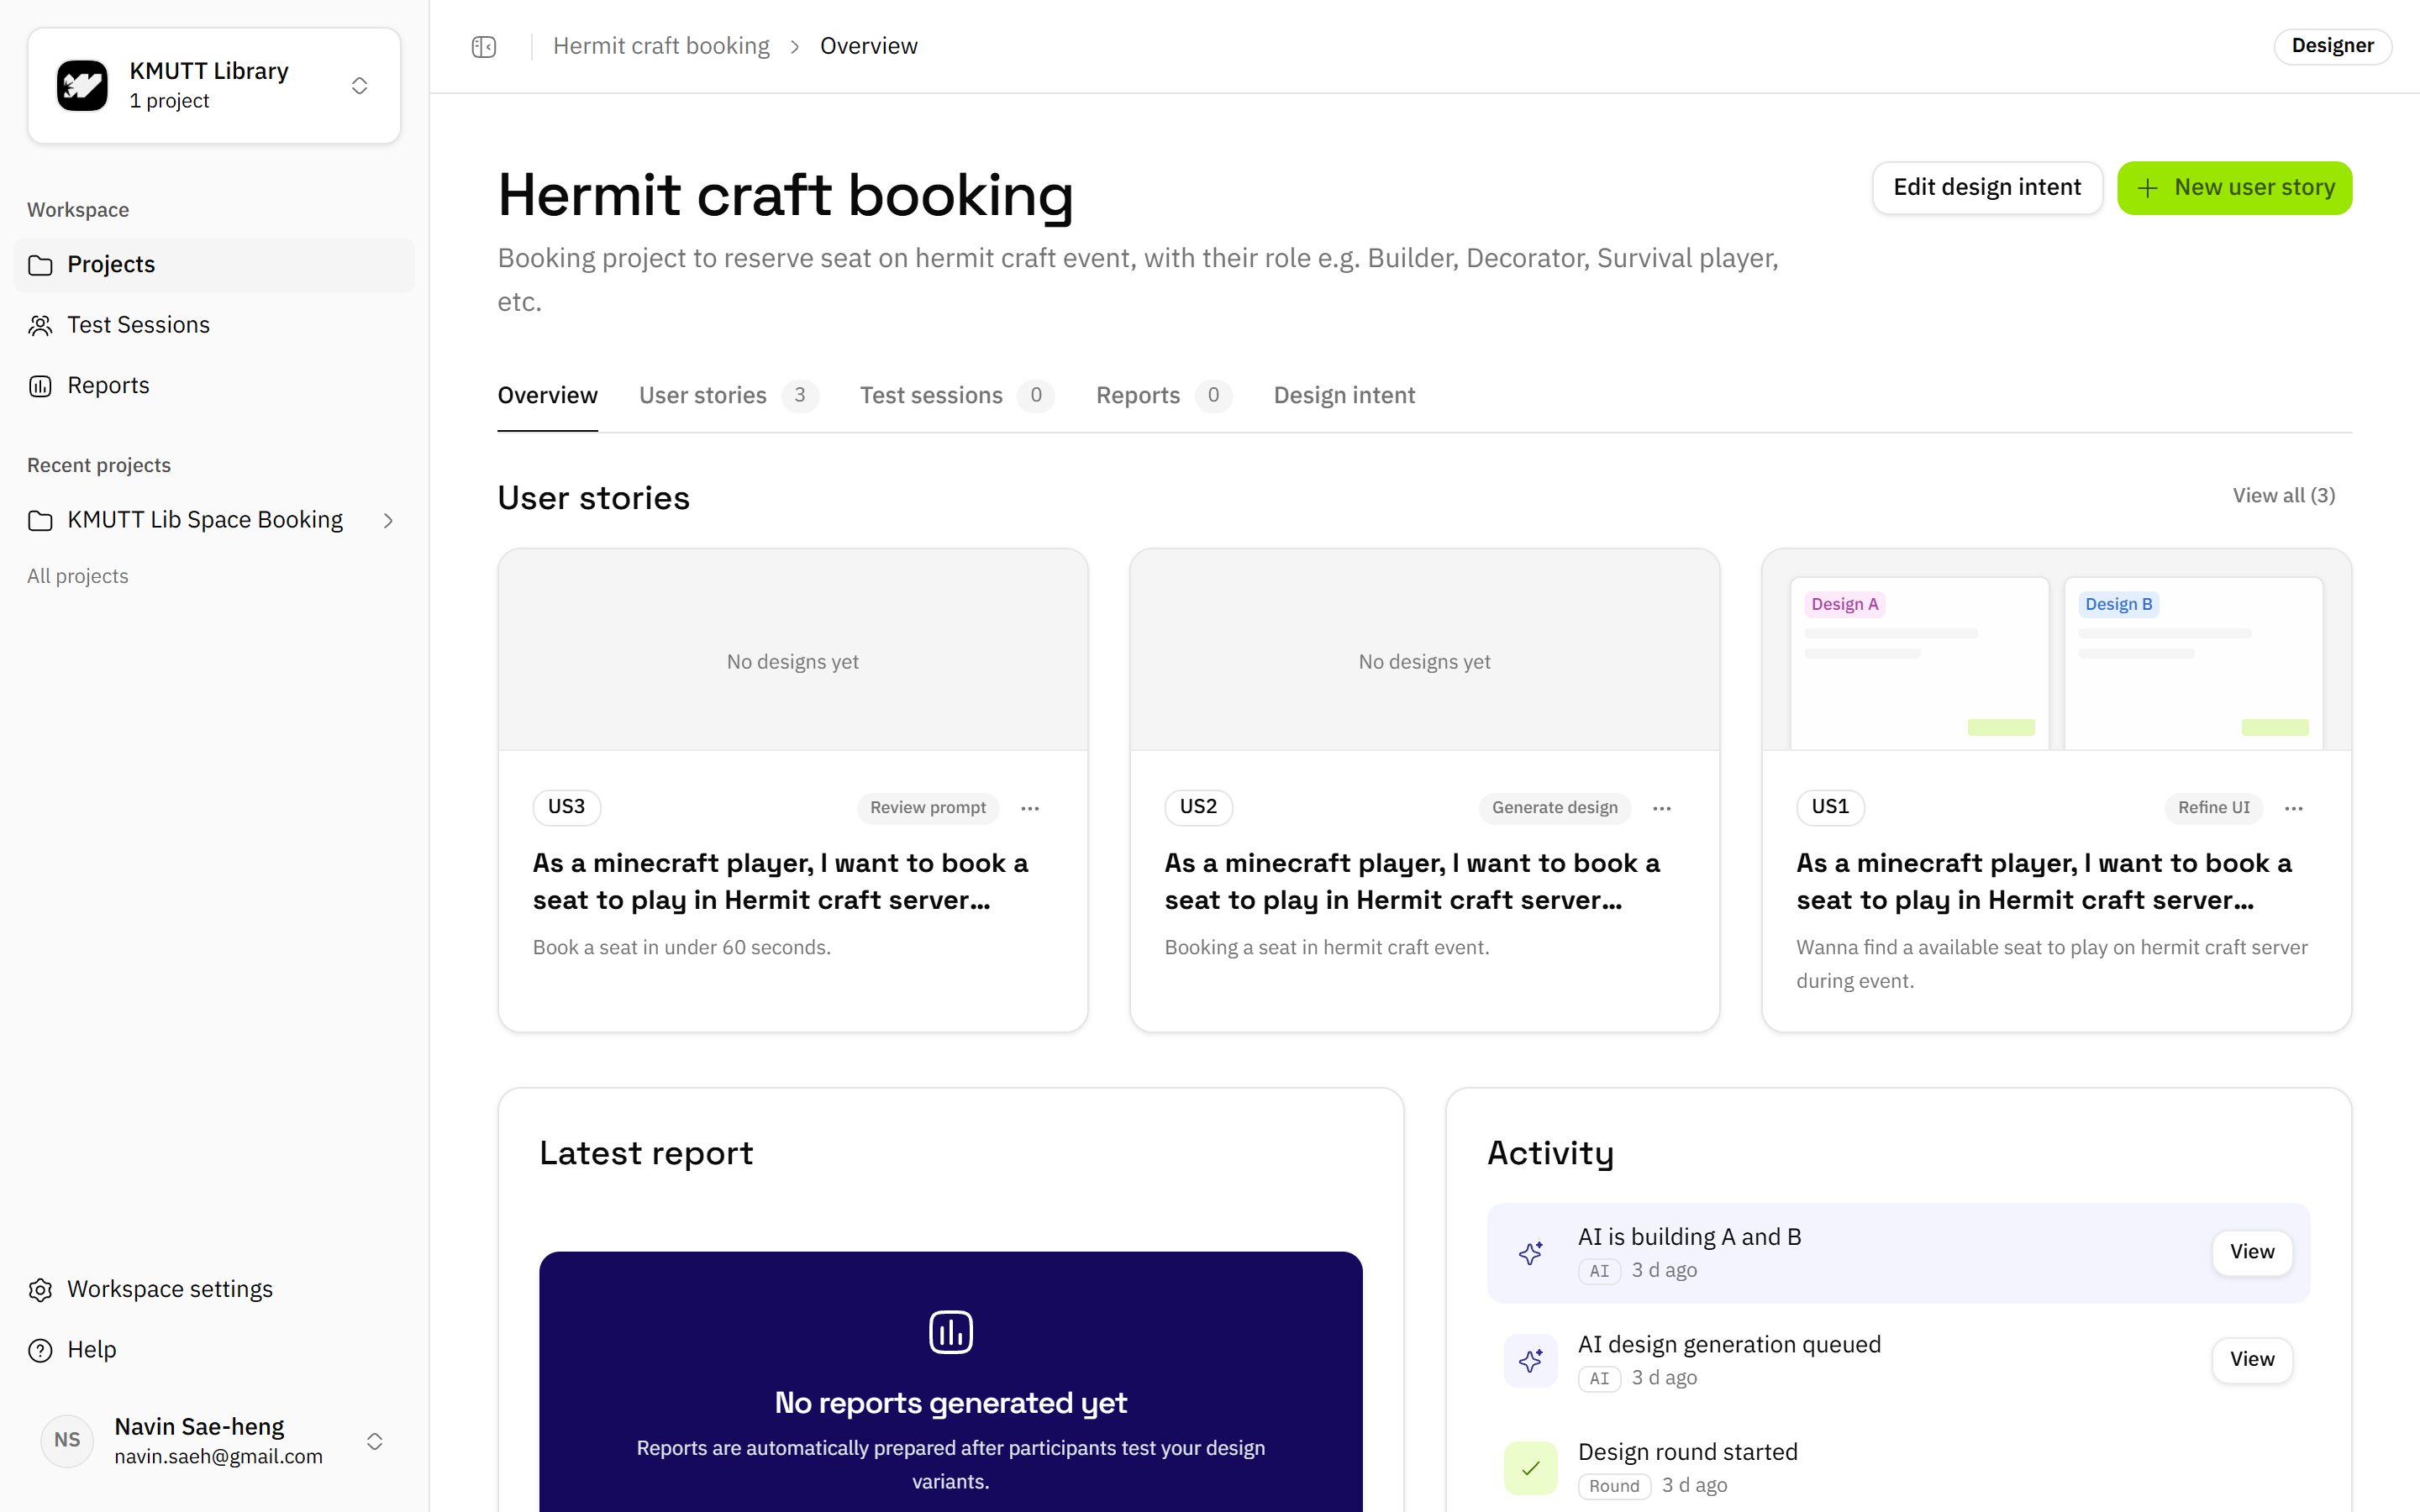
\includegraphics[width=0.9\linewidth]{figures/ch3-methodology/screens/project-overview.png}
  \caption{หน้าภาพรวมของโปรเจกต์ แสดง user story และกิจกรรมล่าสุด}
  \label{fig:screen-project-overview}
\end{figure}

\subsection{M3: AI Design Generation}
\thaijustify{
  นักออกแบบเขียน user story และ problem statement ผ่านหน้าจอ ซึ่ง backend รองรับการให้ AI ร่าง user story แล้วแต่ยังไม่มีหน้าจอสำหรับส่วนนี้ จากนั้น AI ร่าง structured prompt จาก design intent, persona และ user story และส่งผลลัพธ์พร้อมความคิดของโมเดลมาแสดงแบบ real-time ผ่าน SSE นักออกแบบเลือก persona ตรวจ และแก้ prompt ก่อนสั่งสร้าง UI (รูปที่~\ref{fig:screen-story} และ~\ref{fig:screen-prompt})
}
\begin{figure}[H]
  \centering
  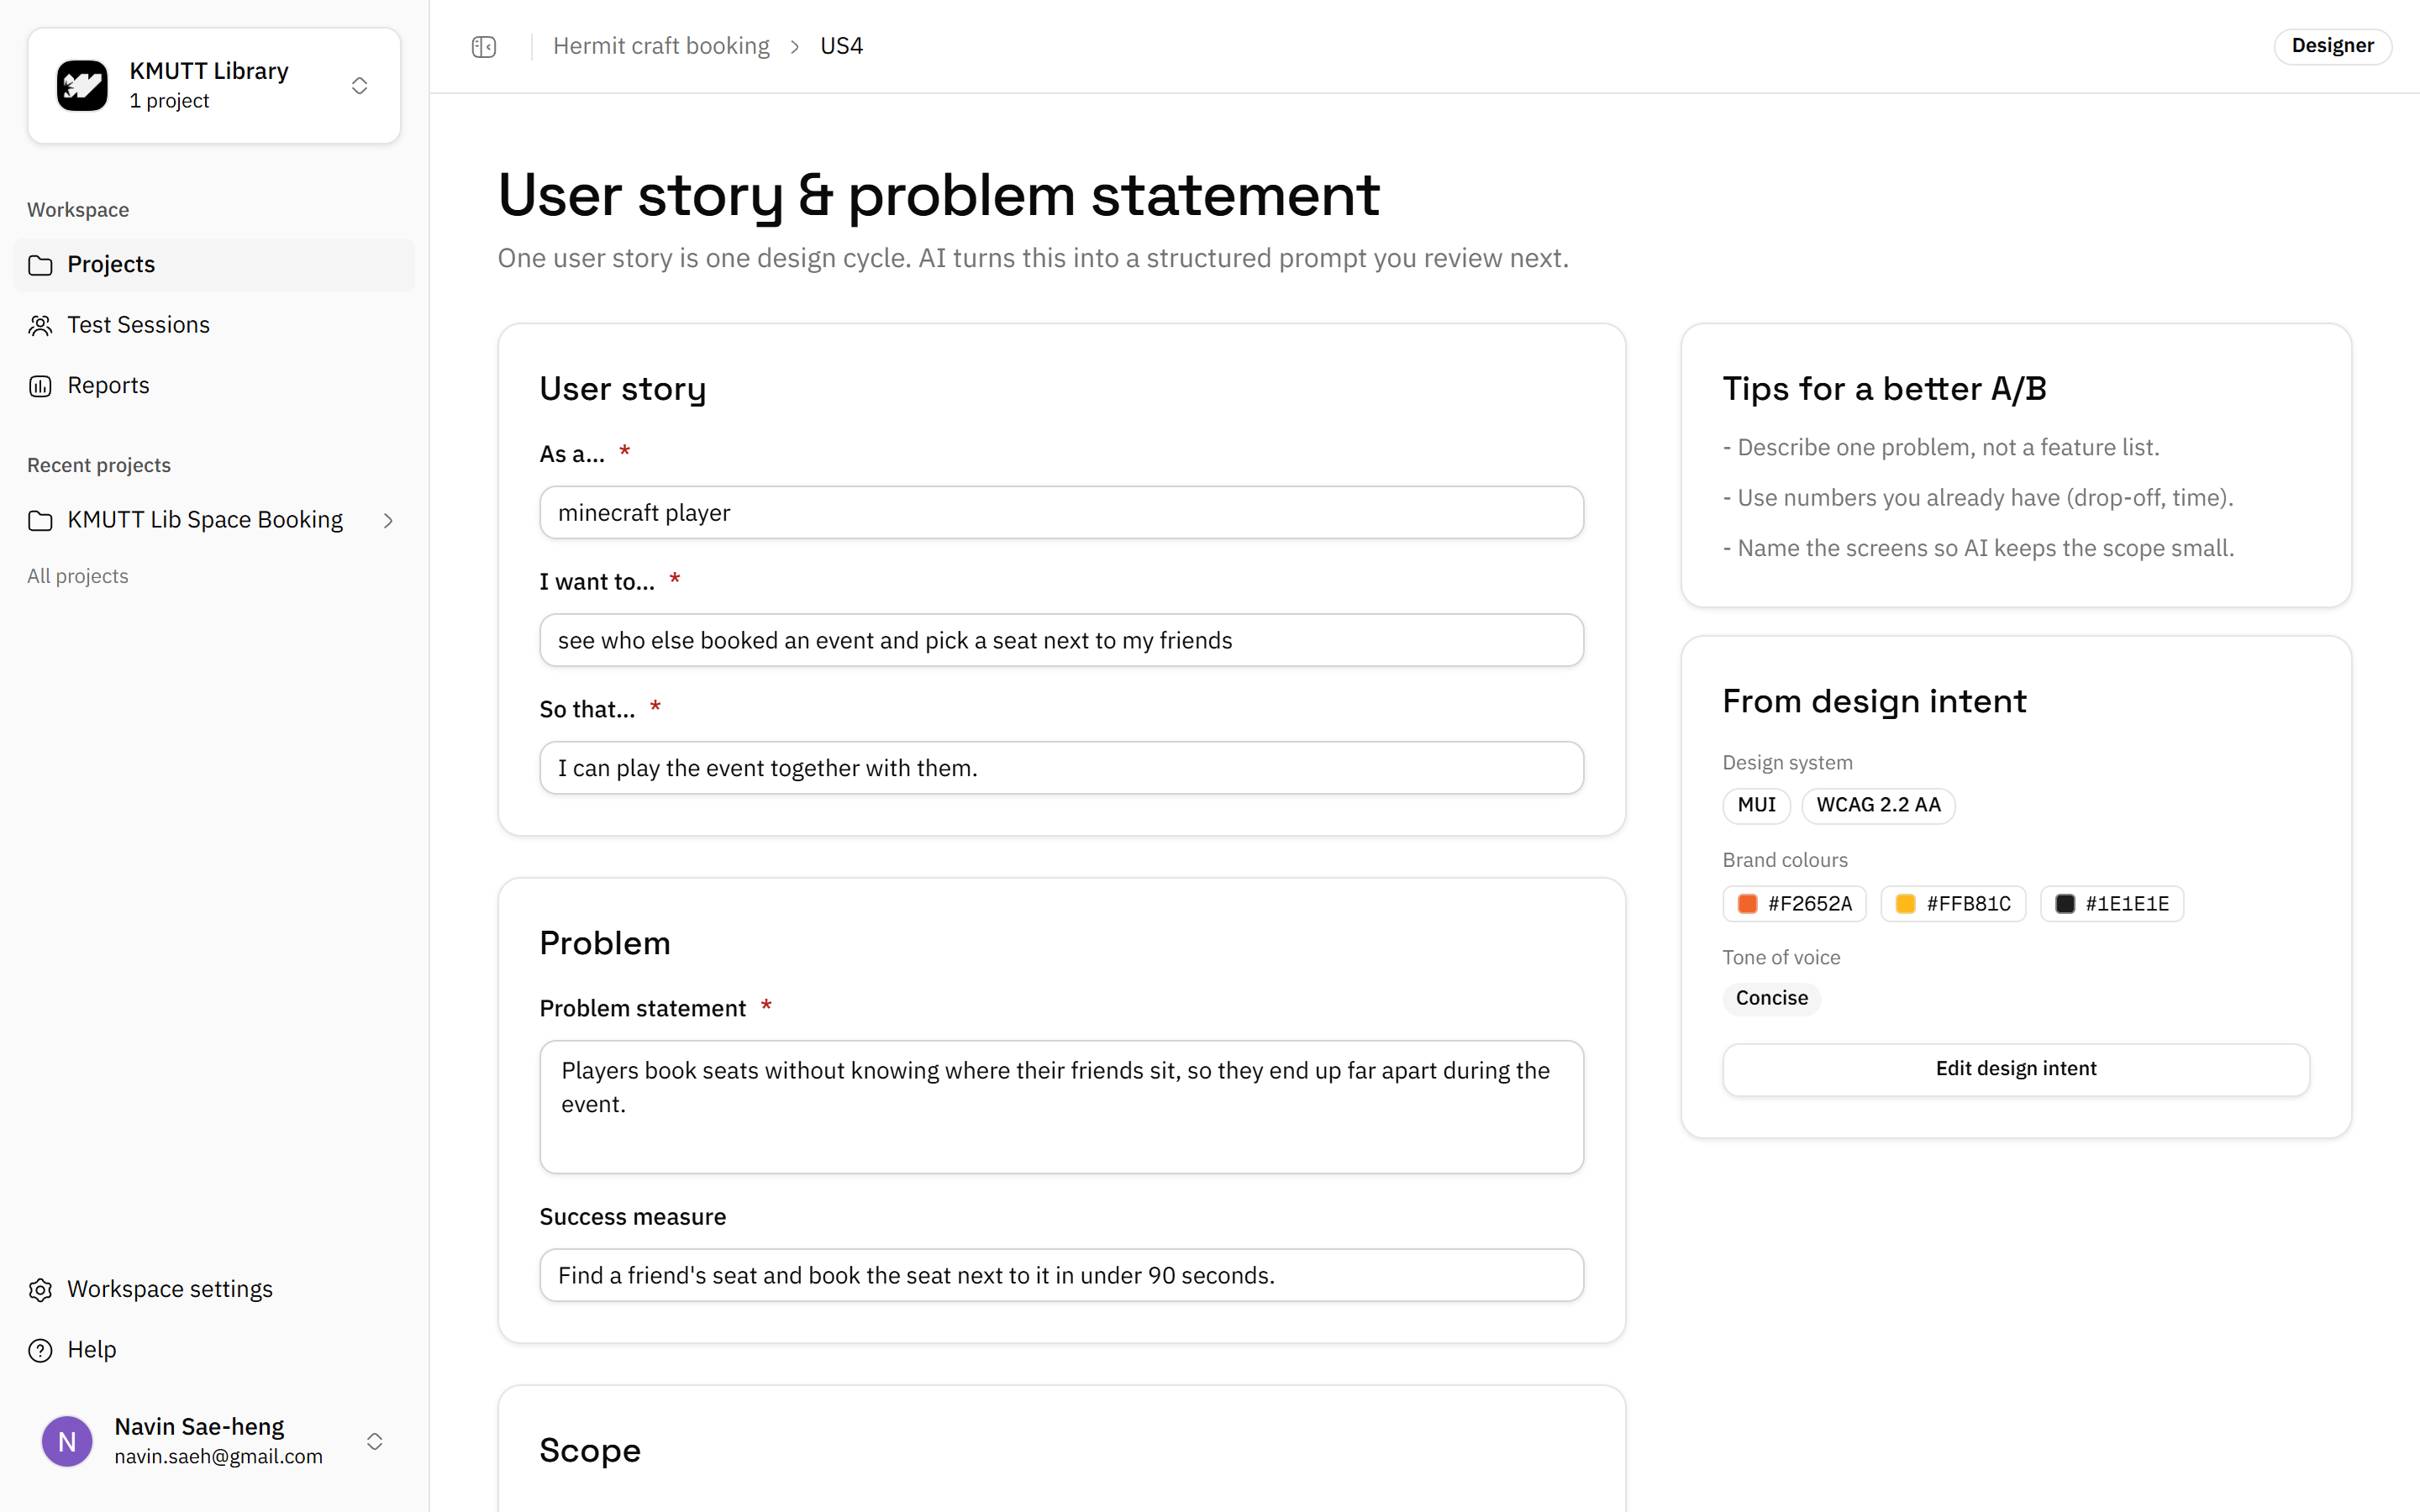
\includegraphics[width=0.9\linewidth]{figures/ch3-methodology/screens/story-us4.png}
  \caption{หน้าจอเขียน user story และ problem statement}
  \label{fig:screen-story}
\end{figure}
\begin{figure}[H]
  \centering
  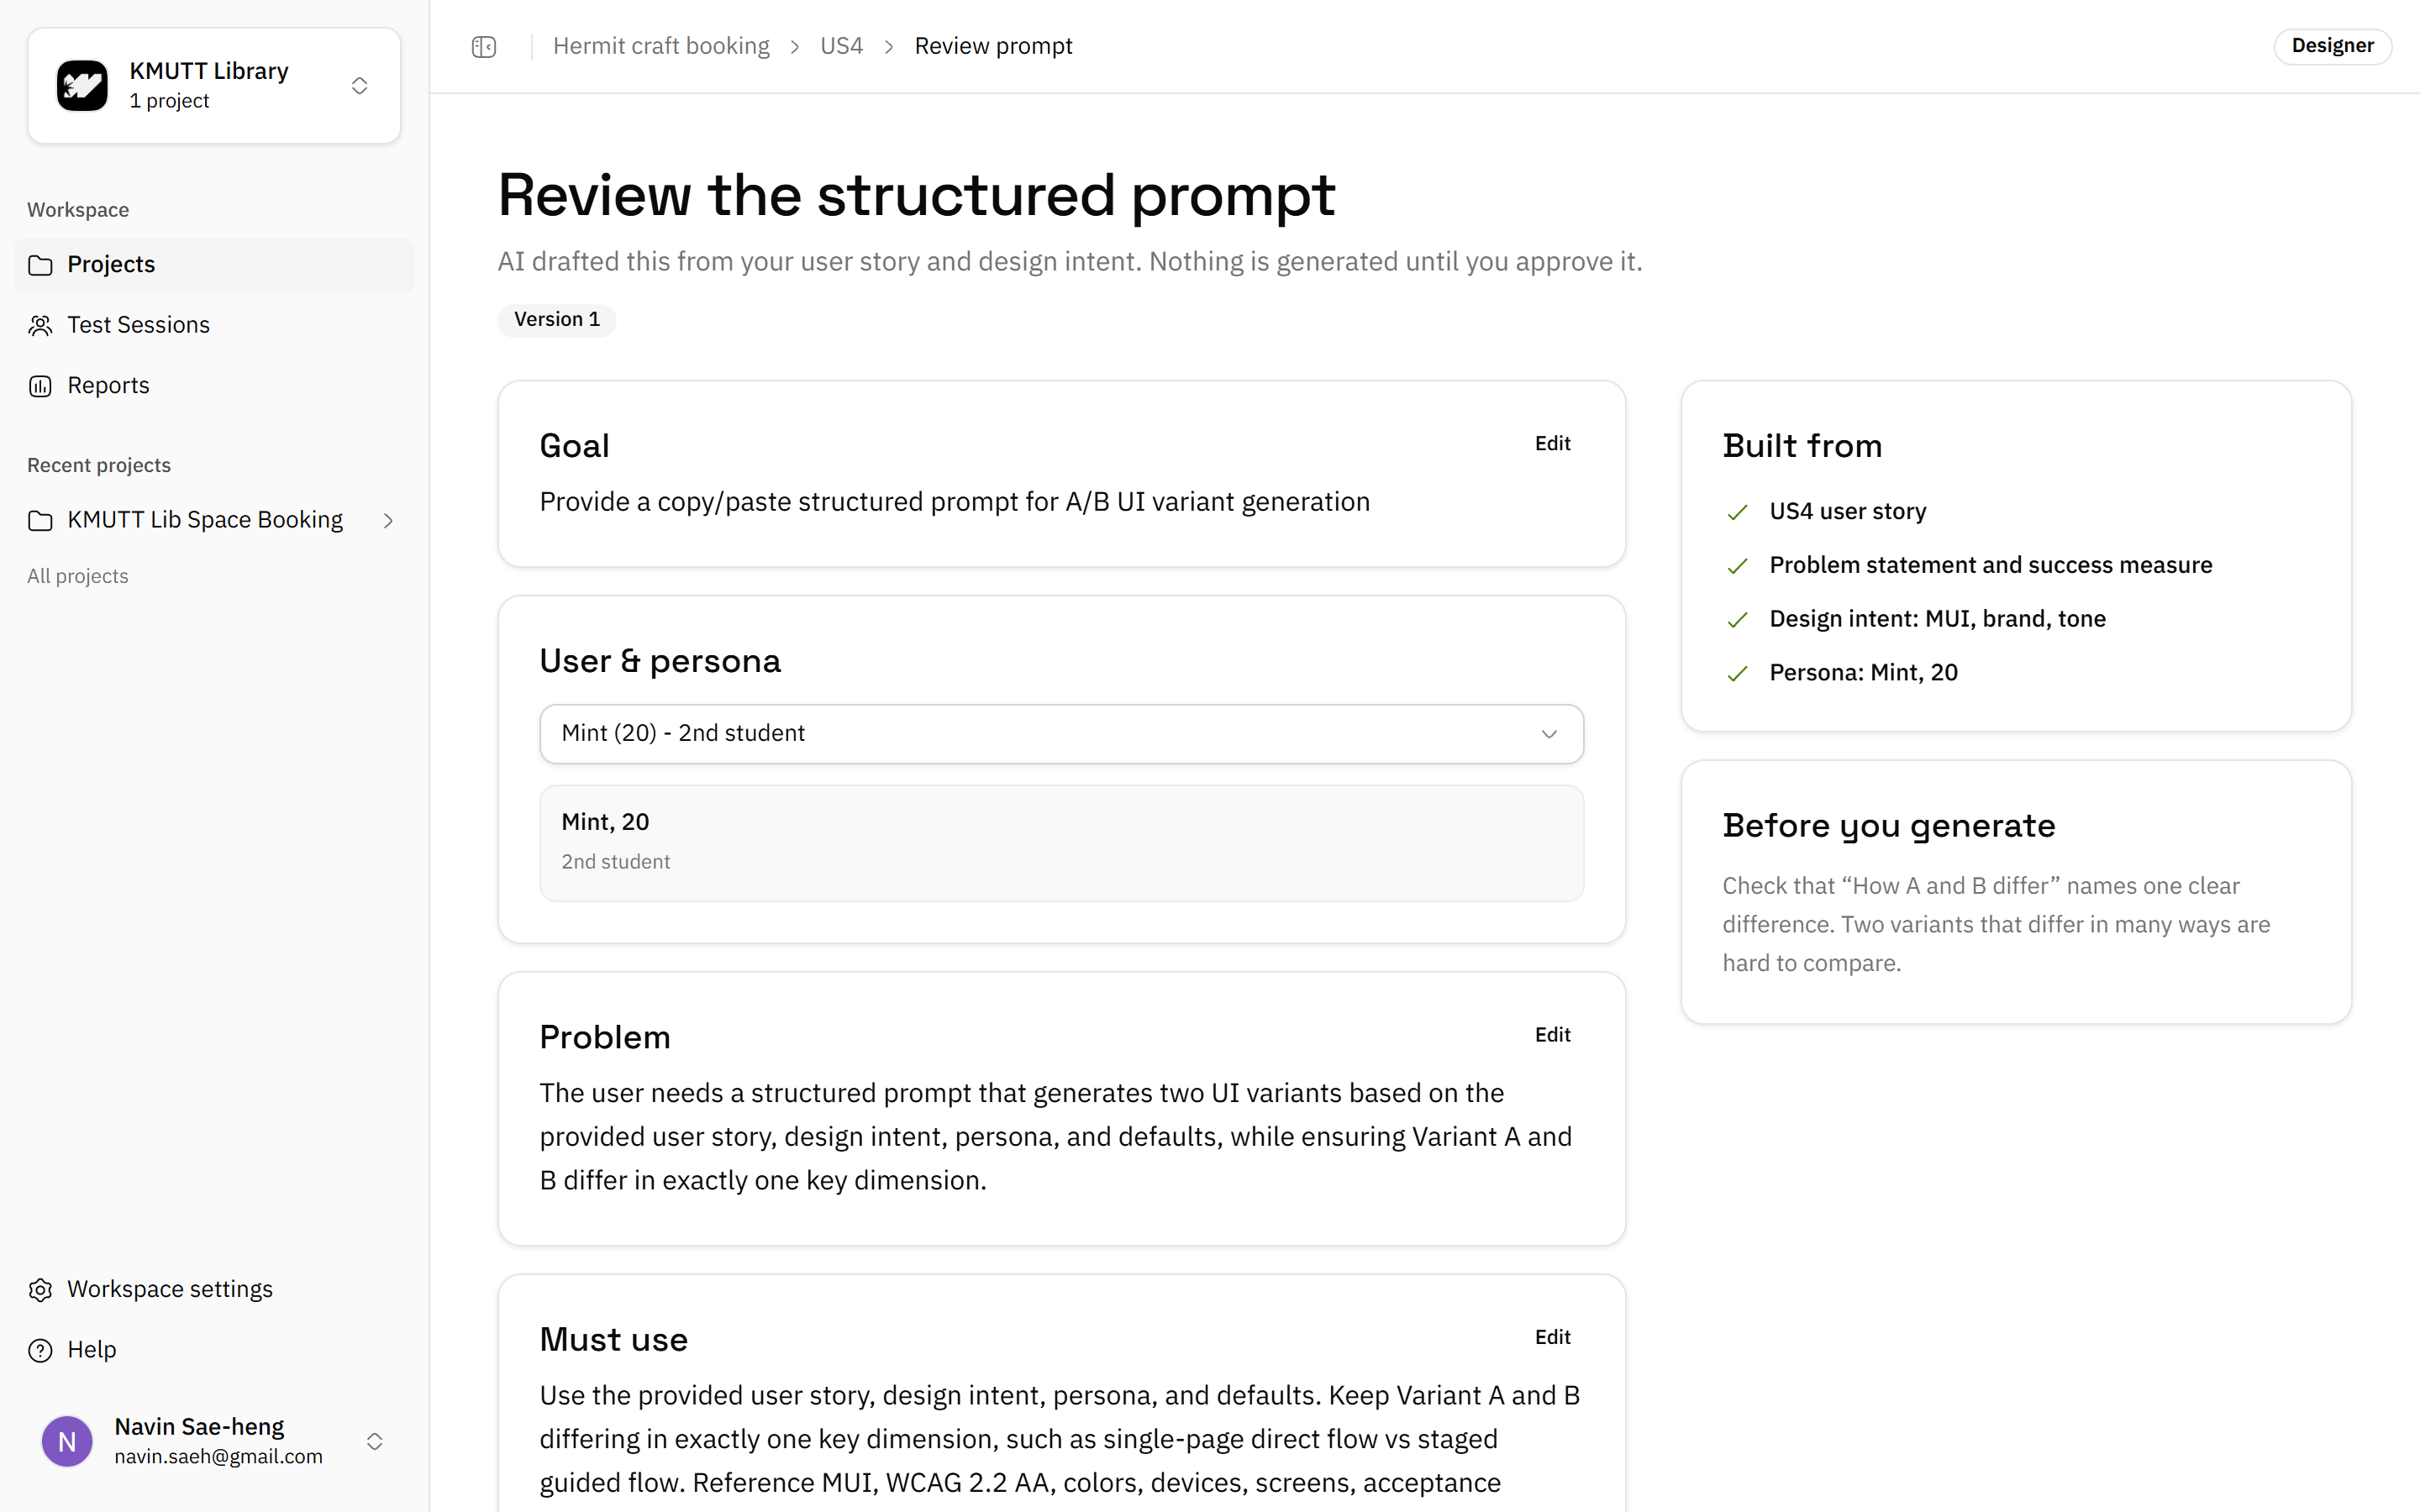
\includegraphics[width=0.9\linewidth]{figures/ch3-methodology/screens/prompt.png}
  \caption{หน้าจอตรวจ structured prompt ที่ AI ร่างก่อนสั่งสร้าง variant A และ B}
  \label{fig:screen-prompt}
\end{figure}
\thaijustify{
  จากนั้นระบบสร้าง UI variant ตามขั้นตอนในหัวข้อ~\ref{sec:ai-pipeline} ระหว่างนั้นหน้าจอแสดง generation trace แบบ real-time (รูปที่~\ref{fig:screen-generate-trace}) และนักออกแบบยกเลิกงานได้
}
\thaijustify{
  หลังได้ variant แล้ว นักออกแบบดูตัวอย่างหน้าจอและปรับแก้ผ่านแชต (chat-based refinement) การแก้แต่ละครั้งสร้าง variant เวอร์ชันใหม่ที่อ้างอิงฉบับเดิม จึงย้อนดูเวอร์ชันก่อนหน้าได้ เมื่อพอใจแล้วนักออกแบบอนุมัติ variant เพื่อนำไปทดสอบ สำหรับการกำหนดภารกิจและการเริ่มเซสชันการทดสอบ backend รองรับแล้ว แต่หน้าจอฝั่ง frontend อยู่ในแผนของภาคการศึกษาที่ 2
}
\begin{figure}[H]
  \centering
  \subfloat[Variant A: single-page direct flow]{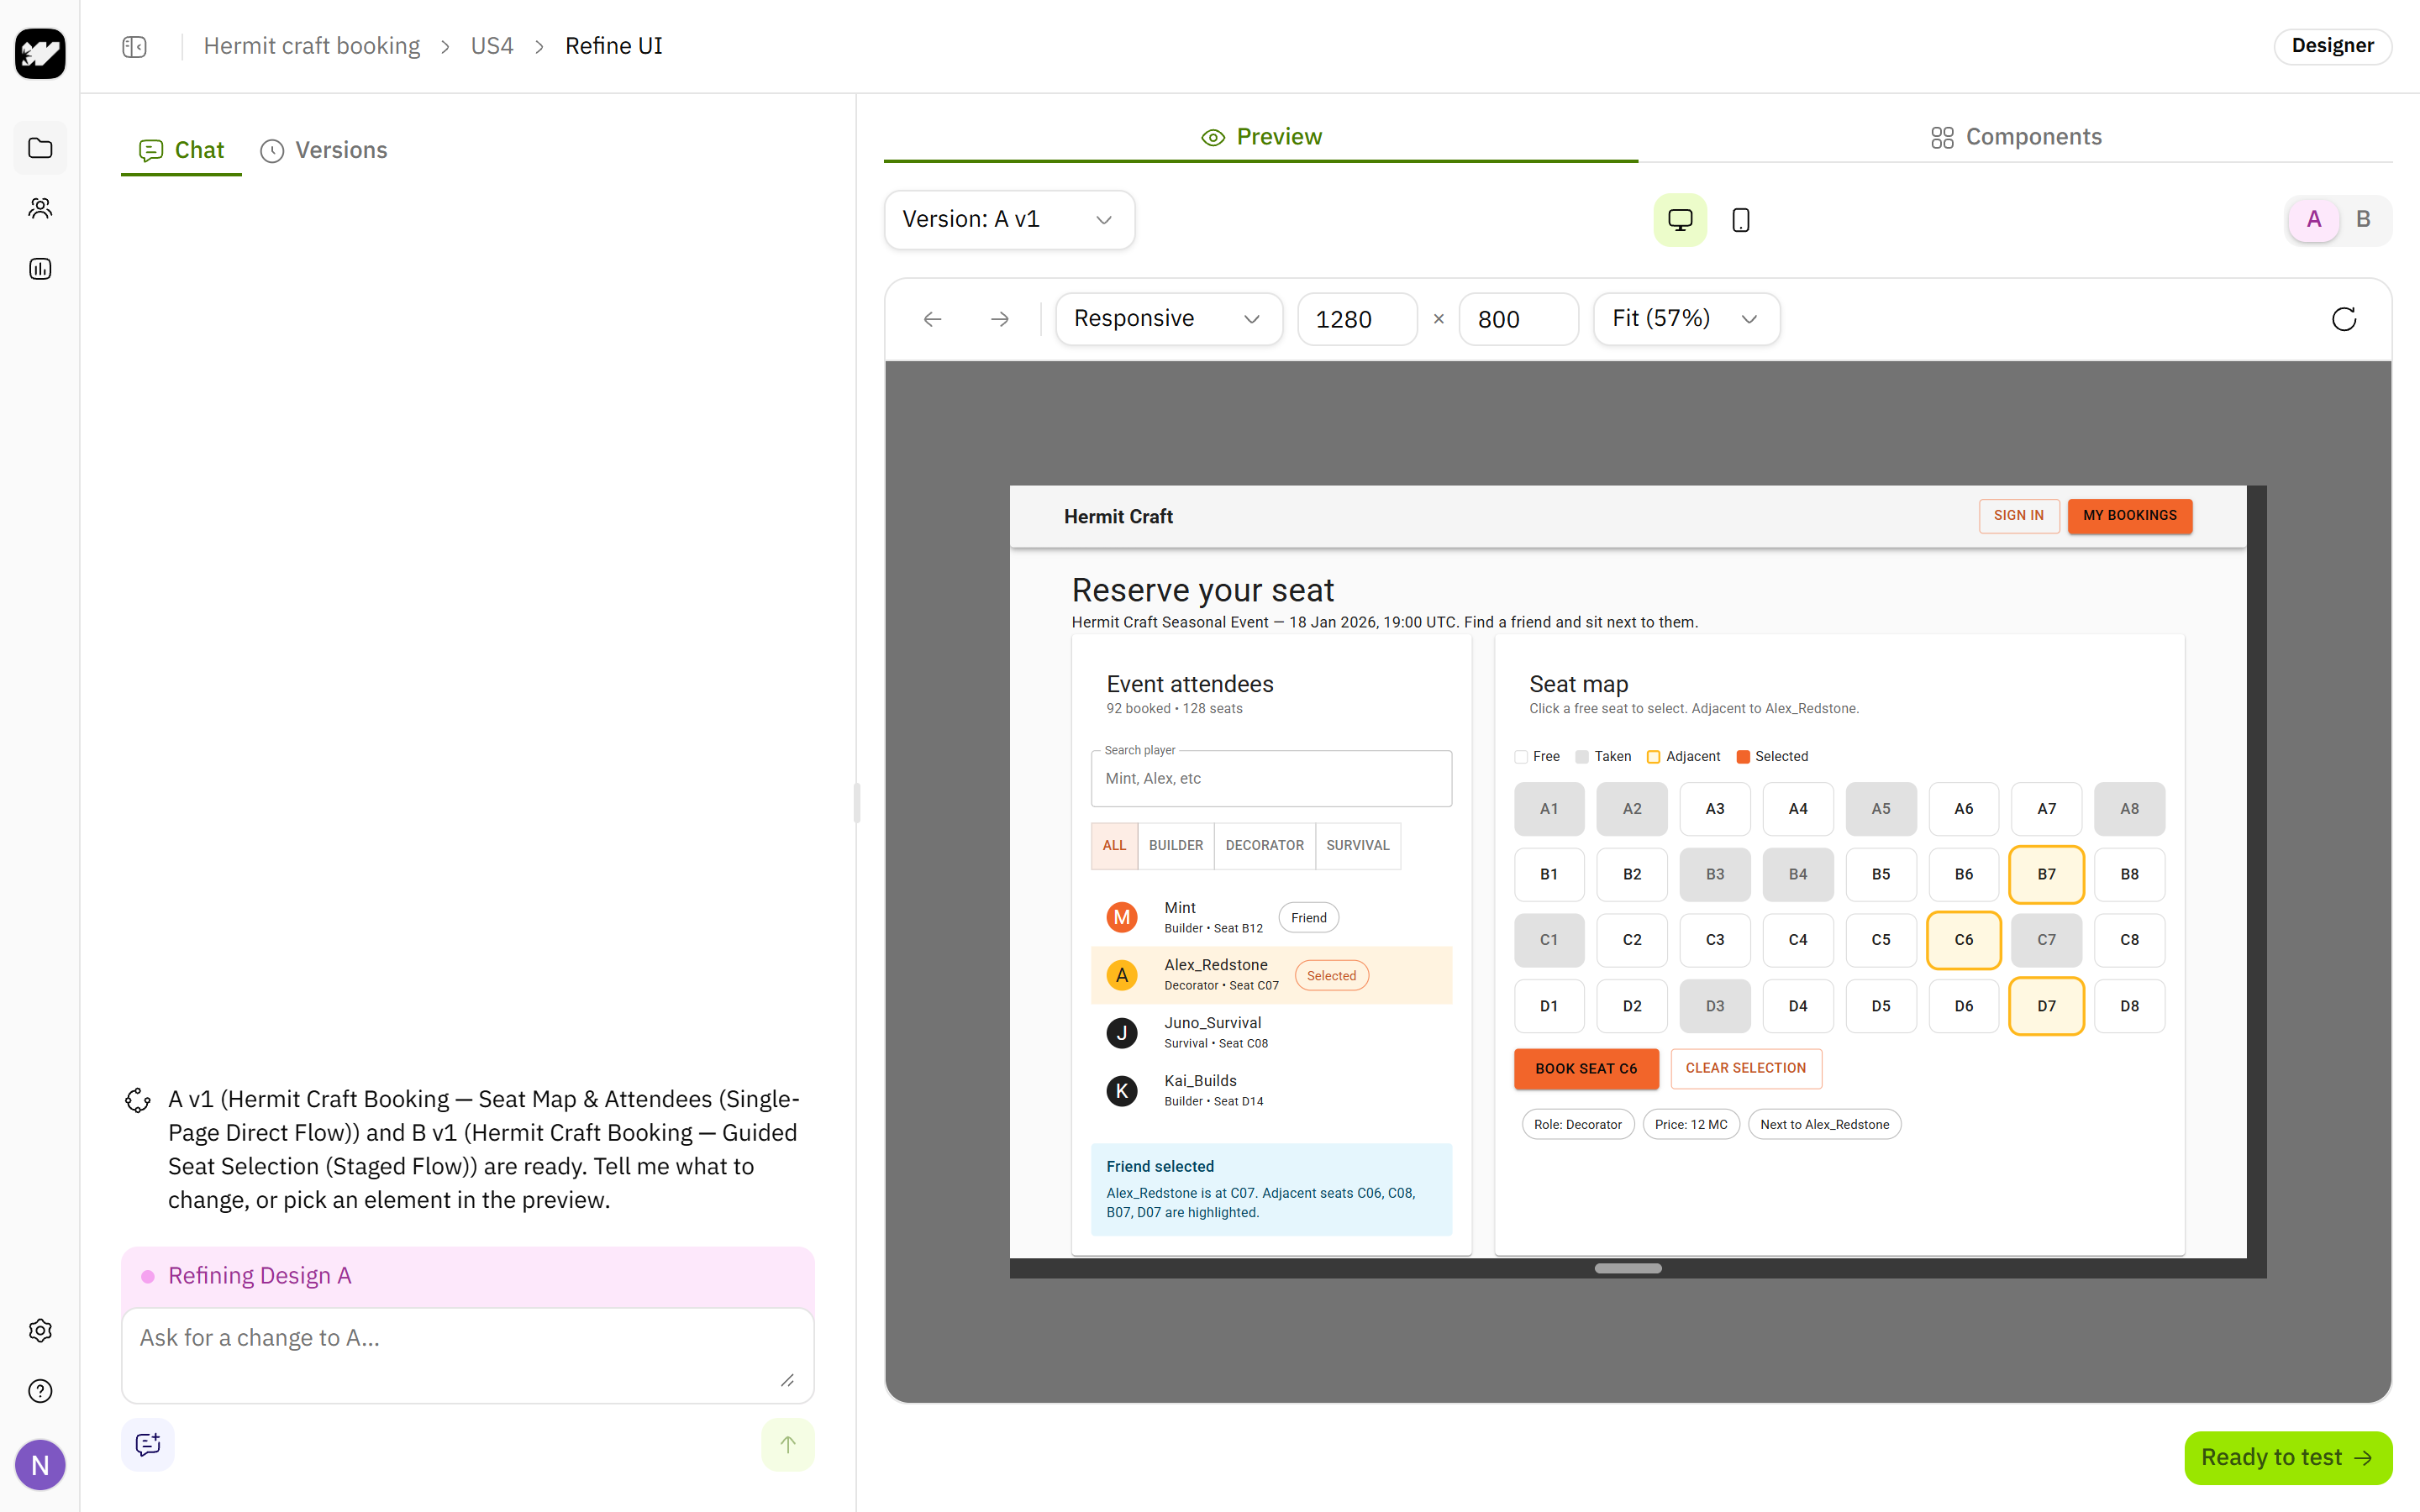
\includegraphics[width=0.49\linewidth]{figures/ch3-methodology/screens/refine-us4.png}}\hfill
  \subfloat[Variant B: staged guided flow]{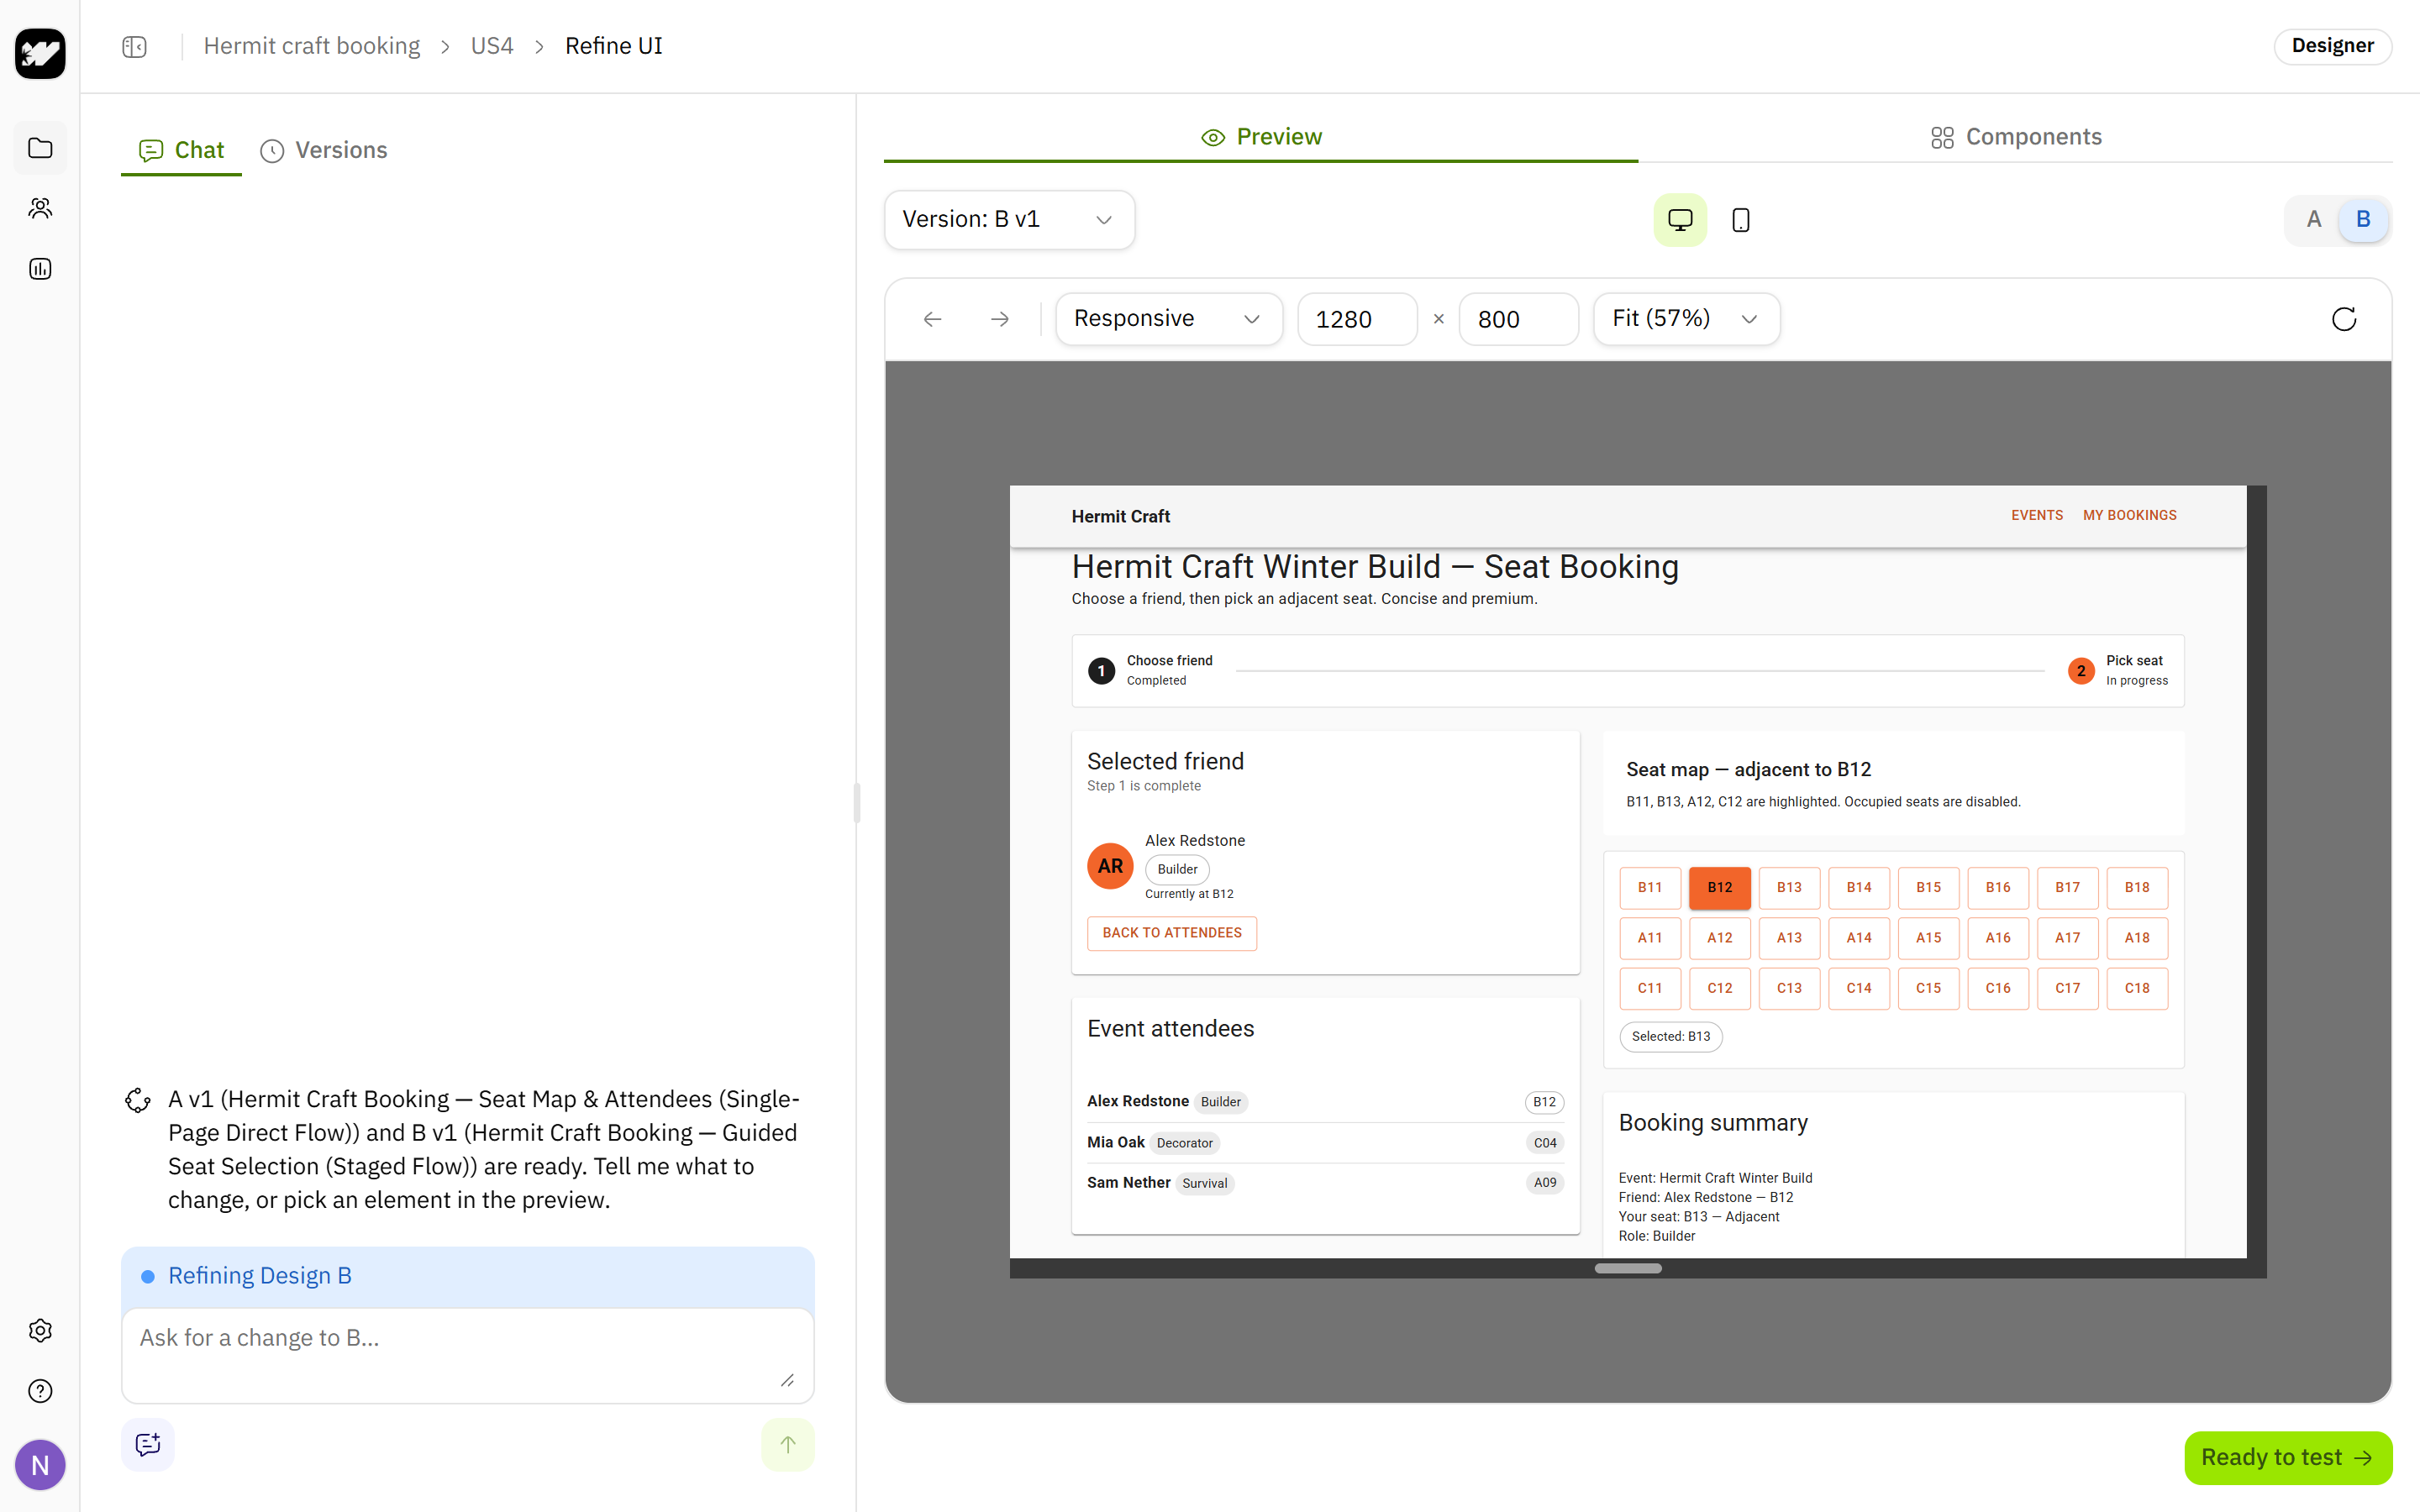
\includegraphics[width=0.49\linewidth]{figures/ch3-methodology/screens/refine-us4-b.png}}
  \caption{หน้าจอปรับแก้ variant ผ่านแชต (ซ้าย) พร้อมหน้าตัวอย่าง (ขวา) ของ two-alternative UI ที่ AI สร้างจาก user story เดียวกัน}
  \label{fig:screen-refine}
\end{figure}

\subsection{Application Program Interface}
\thaijustify{
  Backend ให้บริการผ่าน REST API ที่มีเอกสารแบบ OpenAPI ผ่าน Swagger UI API ส่วนใหญ่ต้องใช้ access token ของผู้ใช้ ส่วน API ของผู้เข้าร่วมทดสอบใช้ token ที่แลกได้จากลิงก์เชิญ ซึ่งมีอายุไม่เกินระยะเวลาของเซสชัน งานที่ใช้เวลานานมี endpoint แบบ SSE สำหรับติดตามความคืบหน้า กลุ่มของ API แสดงในตารางที่~\ref{tab:api-groups}
}
\begingroup
\small
\begin{xltabular}{\linewidth}{|>{\RaggedRight\arraybackslash}p{0.36\linewidth}|>{\RaggedRight\arraybackslash}X|}
  \caption{กลุ่มของ API ในระบบ}\label{tab:api-groups}\\
  \hline
  \textbf{Path} & \textbf{หน้าที่} \\ \hline
  \endfirsthead
  \hline
  \textbf{Path} & \textbf{หน้าที่} \\ \hline
  \endhead
  \texttt{/auth} & เข้าสู่ระบบด้วย Google, ขอ token ใหม่ และออกจากระบบ \\ \hline
  \texttt{/users} & ข้อมูลและรูปโปรไฟล์ของผู้ใช้ \\ \hline
  \texttt{/workspaces} & จัดการ workspace, สมาชิก, คำเชิญ และรูปประจำ workspace \\ \hline
  \texttt{/projects}, \texttt{/projects/:id/members} & จัดการโปรเจกต์และสมาชิกในโปรเจกต์ \\ \hline
  \texttt{/projects/:id/design-intent}, \texttt{personas}, \texttt{user-stories} & ความต้องการทางการออกแบบ, persona และ user story \\ \hline
  \texttt{/projects/:id/story-generations} & ให้ AI ร่าง user story (มี SSE) \\ \hline
  \texttt{/projects/:id/rounds} & รอบการออกแบบ, การร่าง prompt (SSE) และการอนุมัติรอบ \\ \hline
  \texttt{/projects/:id/rounds/:id/generation-jobs} & สั่ง ติดตาม (SSE) และยกเลิกงานสร้าง UI \\ \hline
  \texttt{/projects/:id/variants} & ดู ปรับแก้ อนุมัติ และดูประวัติเวอร์ชันของ variant \\ \hline
  \texttt{/projects/:id/test-sessions} & เซสชันการทดสอบ ภารกิจ ผู้เข้าร่วม และผลการทดสอบ \\ \hline
  \texttt{/testing} & API ของผู้เข้าร่วมทดสอบ: เข้าร่วม, ให้ความยินยอม, ทำภารกิจ, ส่งพฤติกรรมและข้อเสนอแนะ \\ \hline
  \texttt{/projects/:id/analyses}, \texttt{themes} & วิเคราะห์ข้อเสนอแนะด้วย AI และจัดการประเด็น \\ \hline
  \texttt{/projects/:id/rounds/:id/iterate}, \texttt{decisions} & เริ่มรอบถัดไปจากประเด็นที่เลือก และประวัติการตัดสินใจ \\ \hline
  \texttt{/projects/:id/shared-rounds}, \texttt{handoff}, \texttt{status}, \texttt{reports} & มุมมองและรายงานของ Client, Developer และ Project Manager \\ \hline
  \texttt{/projects/:id/audit-logs}, \texttt{/health} & บันทึกกิจกรรม และตรวจสถานะระบบ \\ \hline
\end{xltabular}
\endgroup
\thaijustify{
  API กลุ่มเซสชันการทดสอบ การวิเคราะห์ข้อเสนอแนะ และรายงาน พัฒนาส่วน backend ไว้ล่วงหน้าแล้ว ส่วนหน้าจอที่ใช้ API เหล่านี้อยู่ในแผนของภาคการศึกษาที่ 2
}
\begin{figure}[H]
  \centering
  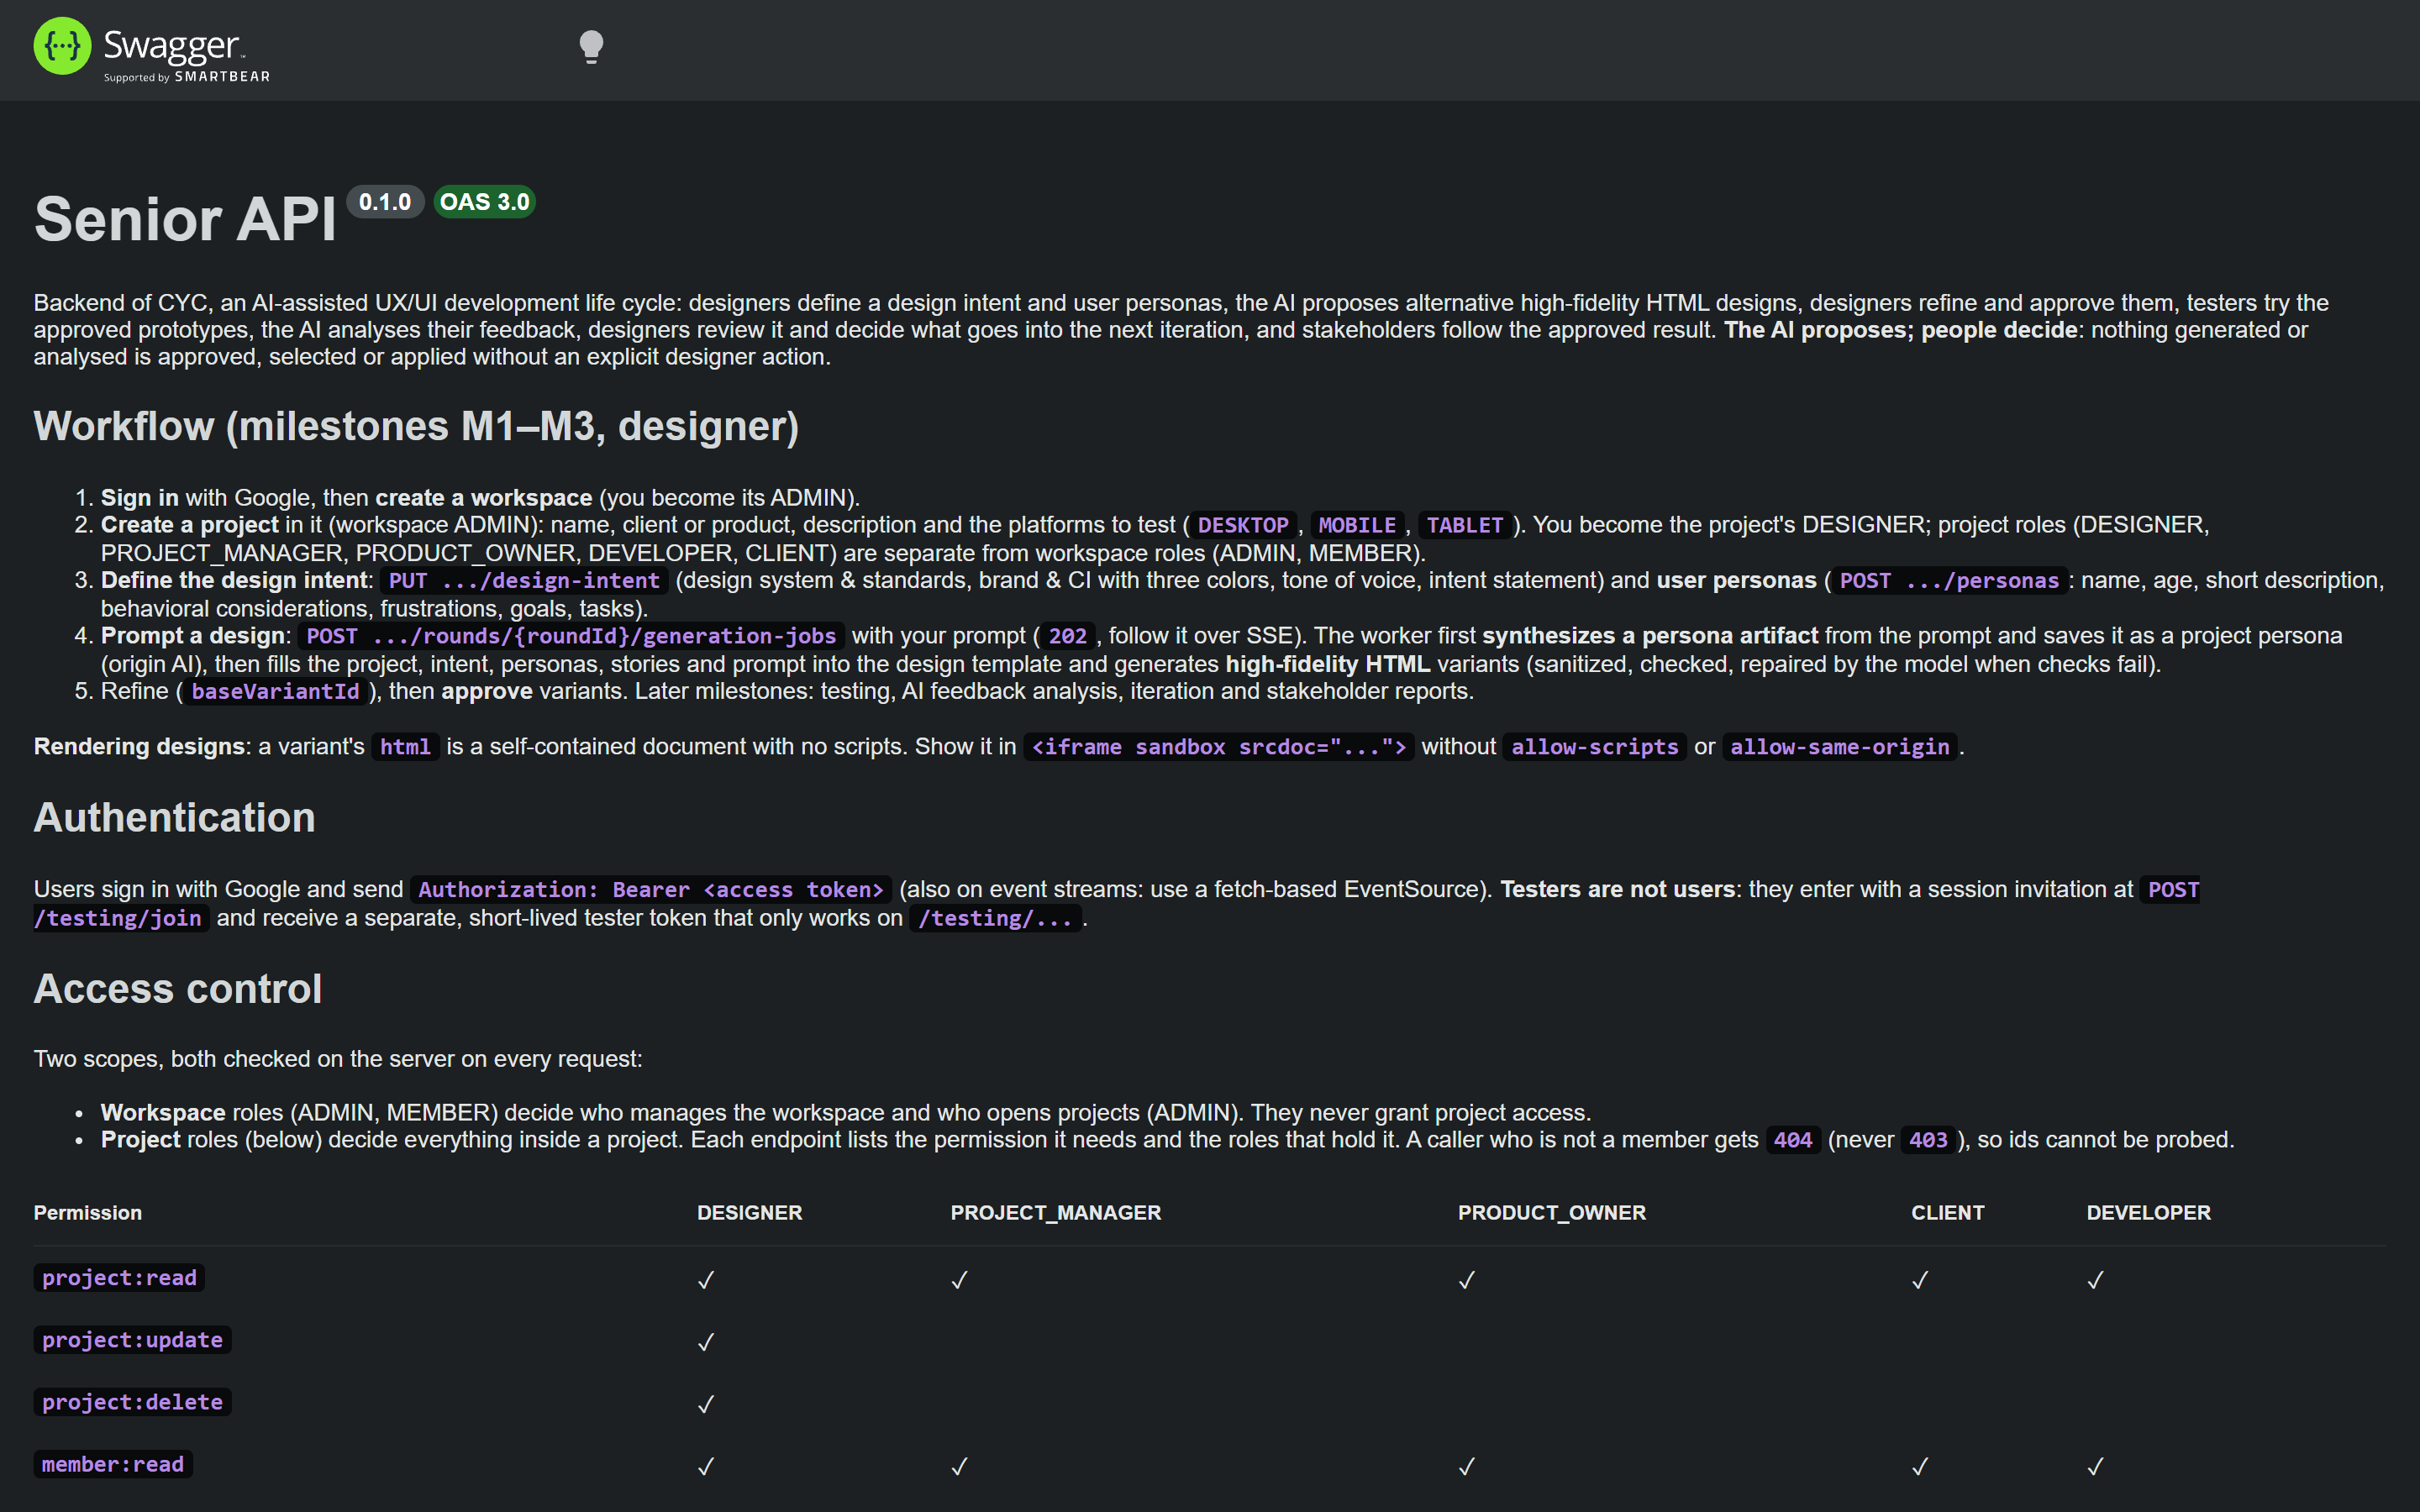
\includegraphics[width=0.9\linewidth]{figures/ch3-methodology/screens/swagger.png}
  \caption{เอกสาร API ผ่าน Swagger UI}
  \label{fig:screen-swagger}
\end{figure}

% !TeX root = ../../progress-sem1.tex
% Subsections of "การพัฒนาระบบ": developed screens per user group, matching
% "การพัฒนาหน้าจอเว็บไซต์ของ Admin / General User" in the example.
% Input from chapters/03-methodology.tex, after the API subsection.

\subsection{การพัฒนาหน้าจอเว็บไซต์ของ Designer}
\thaijustify{
  หน้าจอที่พัฒนาแล้วใน frontend เรียงตามลำดับการใช้งานของนักออกแบบ แสดงในตารางที่~\ref{tab:designer-screens}
}
\begingroup
\small
\begin{xltabular}{\linewidth}{|>{\RaggedRight\arraybackslash}p{0.40\linewidth}|>{\RaggedRight\arraybackslash}X|}
  \caption{หน้าจอของ Designer ที่พัฒนาแล้ว}\label{tab:designer-screens}\\
  \hline
  \textbf{Route} & \textbf{หน้าที่} \\ \hline
  \endfirsthead
  \hline
  \textbf{Route} & \textbf{หน้าที่} \\ \hline
  \endhead
  \texttt{/signin}, \texttt{/signup}, \texttt{/forgot-password} & เข้าสู่ระบบ สมัครสมาชิก และลืมรหัสผ่าน \\ \hline
  \texttt{/first-run}, \texttt{/workspaces/new} & การใช้งานครั้งแรกและการสร้าง workspace \\ \hline
  \texttt{/dashboard}, \texttt{/projects} & ภาพรวมและรายการโปรเจกต์แบบรายการและแกลเลอรี \\ \hline
  \texttt{/projects/new}, \texttt{.../setup/intent}, \texttt{.../setup/team} & wizard สร้างโปรเจกต์ กำหนด design intent และทีม \\ \hline
  \texttt{.../overview}, \texttt{.../intent}, \texttt{.../team} & ภาพรวมโปรเจกต์ แก้ไข design intent และสมาชิก \\ \hline
  \texttt{.../stories}, \texttt{.../stories/new}, \texttt{.../stories/:storyId} & จัดการ user story และ persona ของ story \\ \hline
  \texttt{.../stories/:storyId/prompt} & ตรวจและแก้ structured prompt ก่อนสร้าง UI \\ \hline
  \texttt{.../rounds/:roundId/generate} & สั่งสร้าง UI และดู generation trace \\ \hline
  \texttt{.../rounds/:roundId/refine} & ดูตัวอย่าง variant และปรับแก้ผ่านแชต \\ \hline
\end{xltabular}
\endgroup
\thaijustify{
  หน้า refine แบ่งเป็นแชตและหน้าตัวอย่างที่ปรับขนาดได้ นักออกแบบปักหมุดความคิดเห็นบนตำแหน่งใดก็ได้ของหน้าตัวอย่างแบบเดียวกับ Figma แล้วส่งหลายหมุดพร้อมกันเป็นคำสั่งปรับแก้ หมุดที่ส่งแล้วแสดงสถานะว่าถูกนำไปใช้ใน variant เวอร์ชันใด แถบด้านข้างย่อเป็น icon rail บนหน้านี้เพื่อเพิ่มพื้นที่แสดงผล
}
\thaijustify{
  ภาพหน้าจอของ wizard สร้างโปรเจกต์ design intent, user story, การตรวจ prompt และหน้า refine แสดงไว้ในหัวข้อ M2 และ M3 (รูปที่~\ref{fig:screen-project-new} ถึง~\ref{fig:screen-refine}) รูปที่~\ref{fig:screen-projects} และ~\ref{fig:screen-refine-pins} แสดงรายการโปรเจกต์และหมุดความคิดเห็นบนหน้า refine
}
\begin{figure}[H]
  \centering
  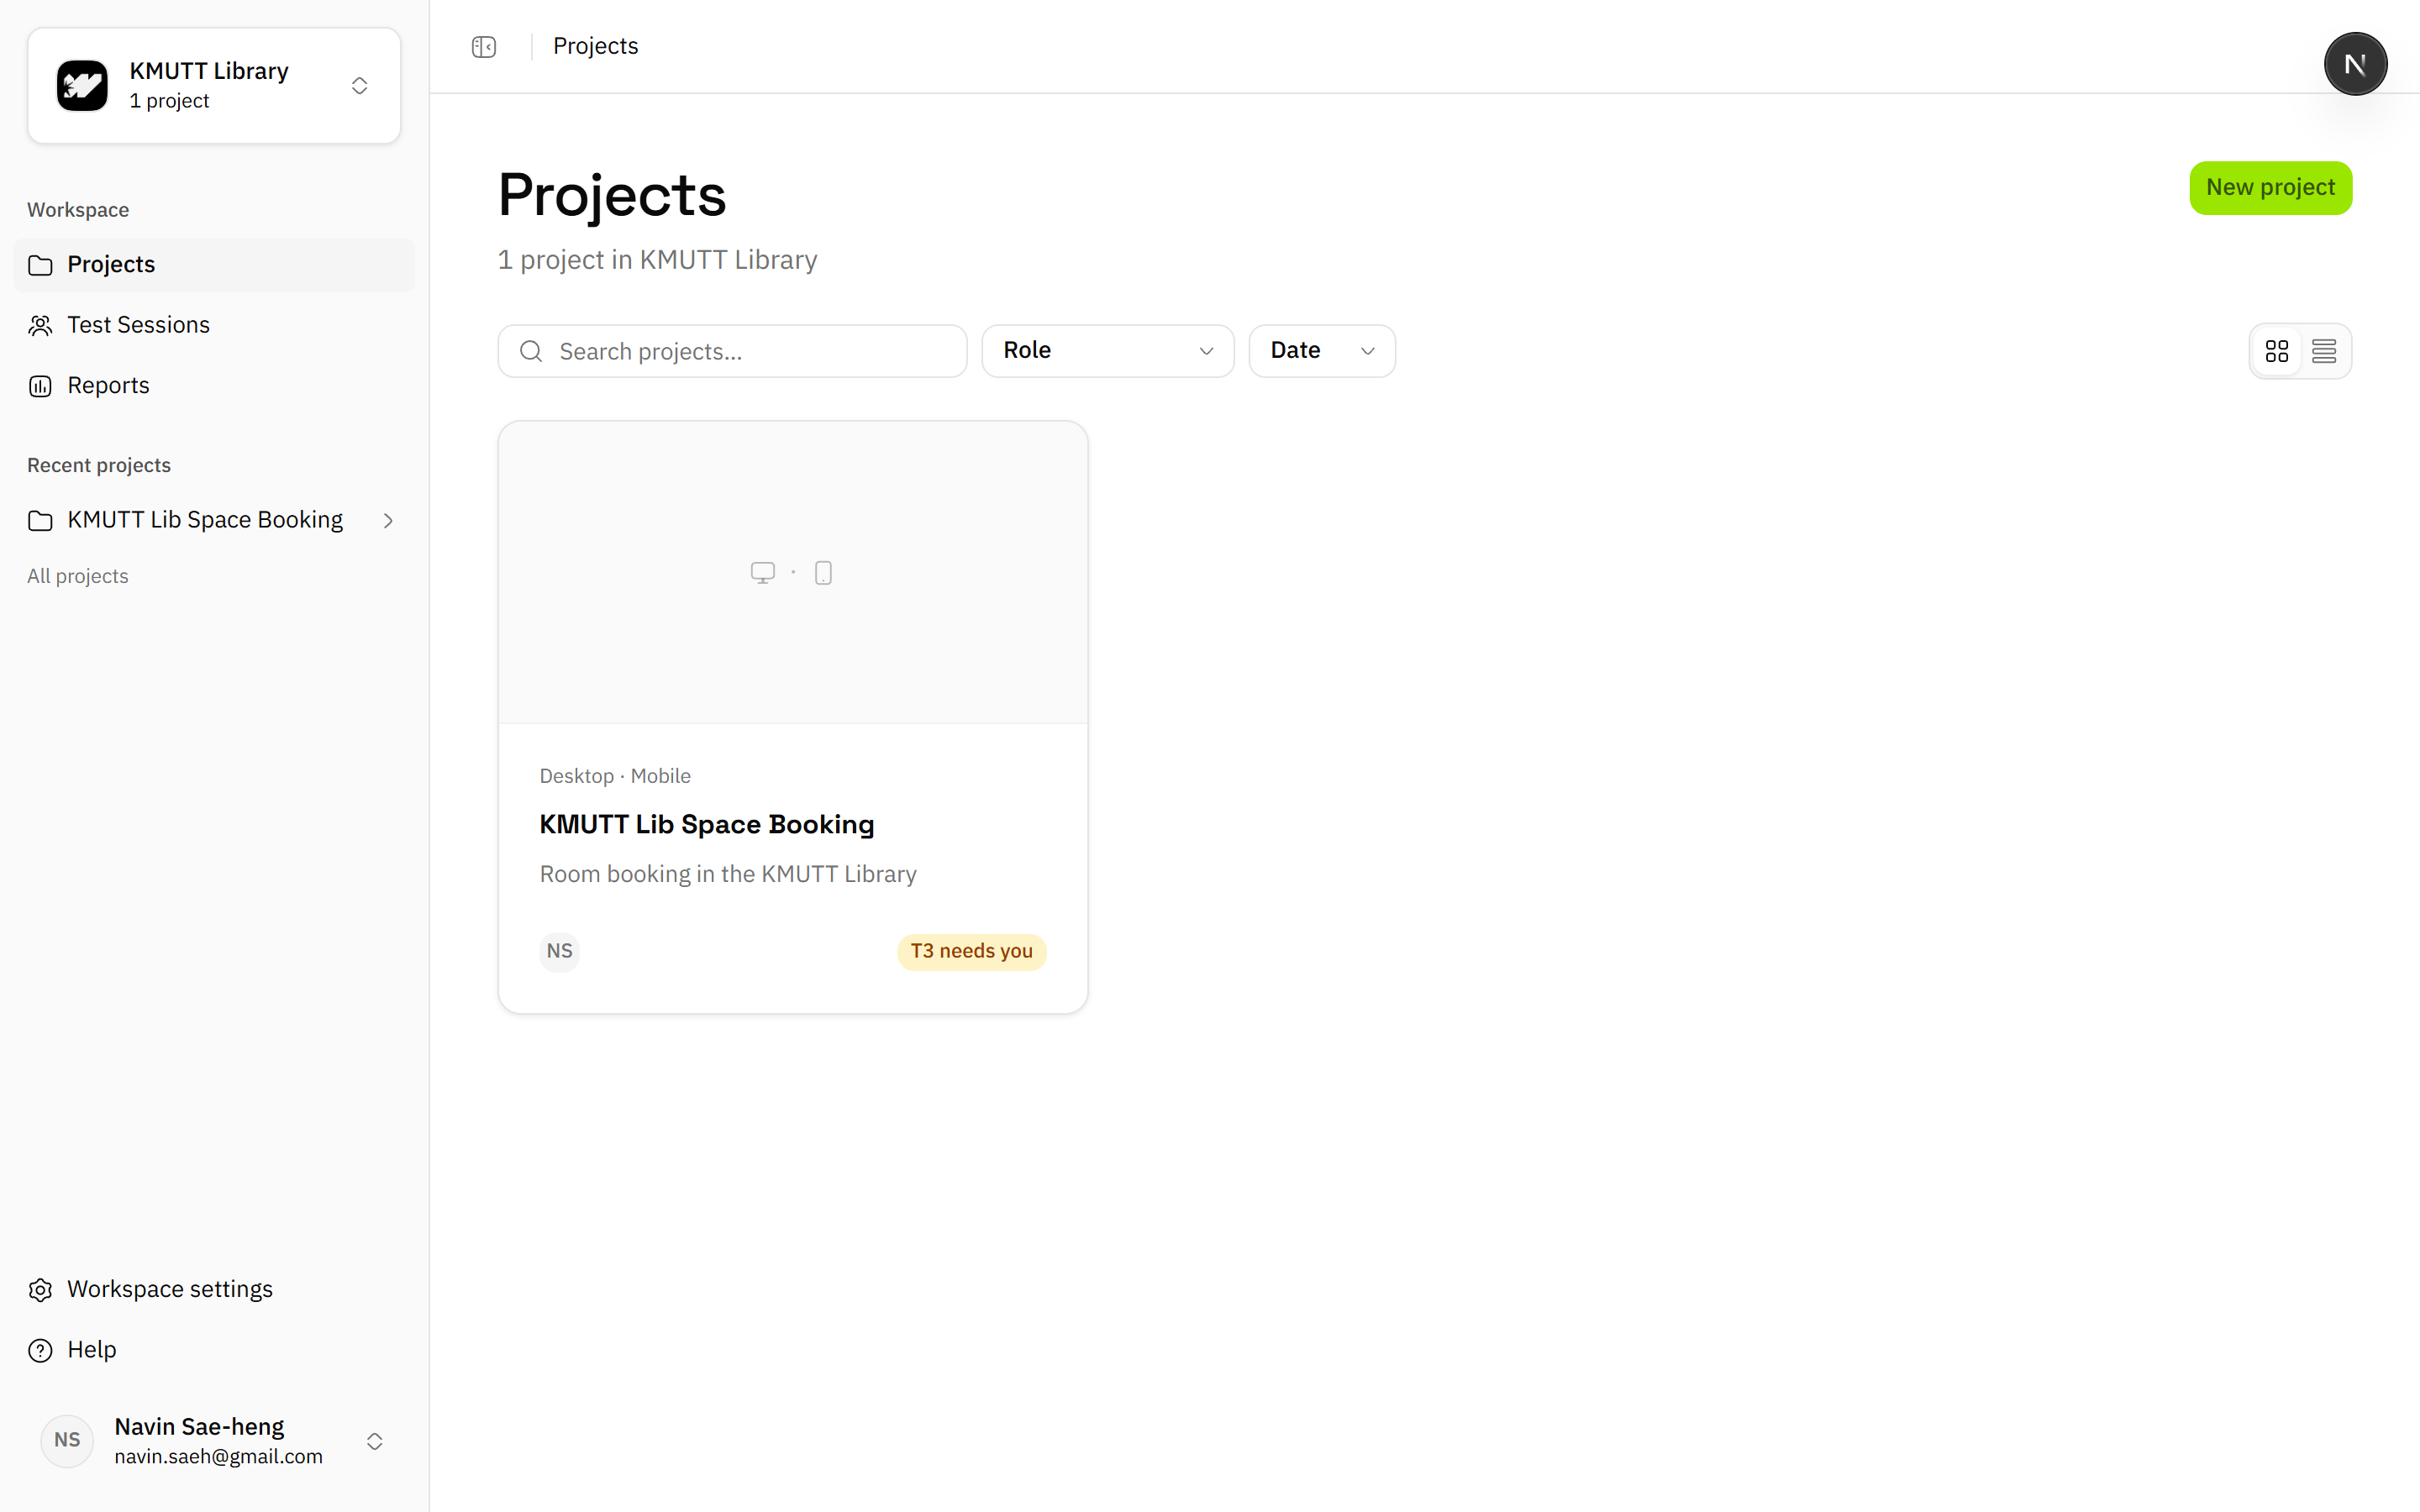
\includegraphics[width=0.9\linewidth]{figures/ch3-methodology/screens/projects.png}
  \caption{หน้ารายการโปรเจกต์ใน workspace}
  \label{fig:screen-projects}
\end{figure}
\begin{figure}[H]
  \centering
  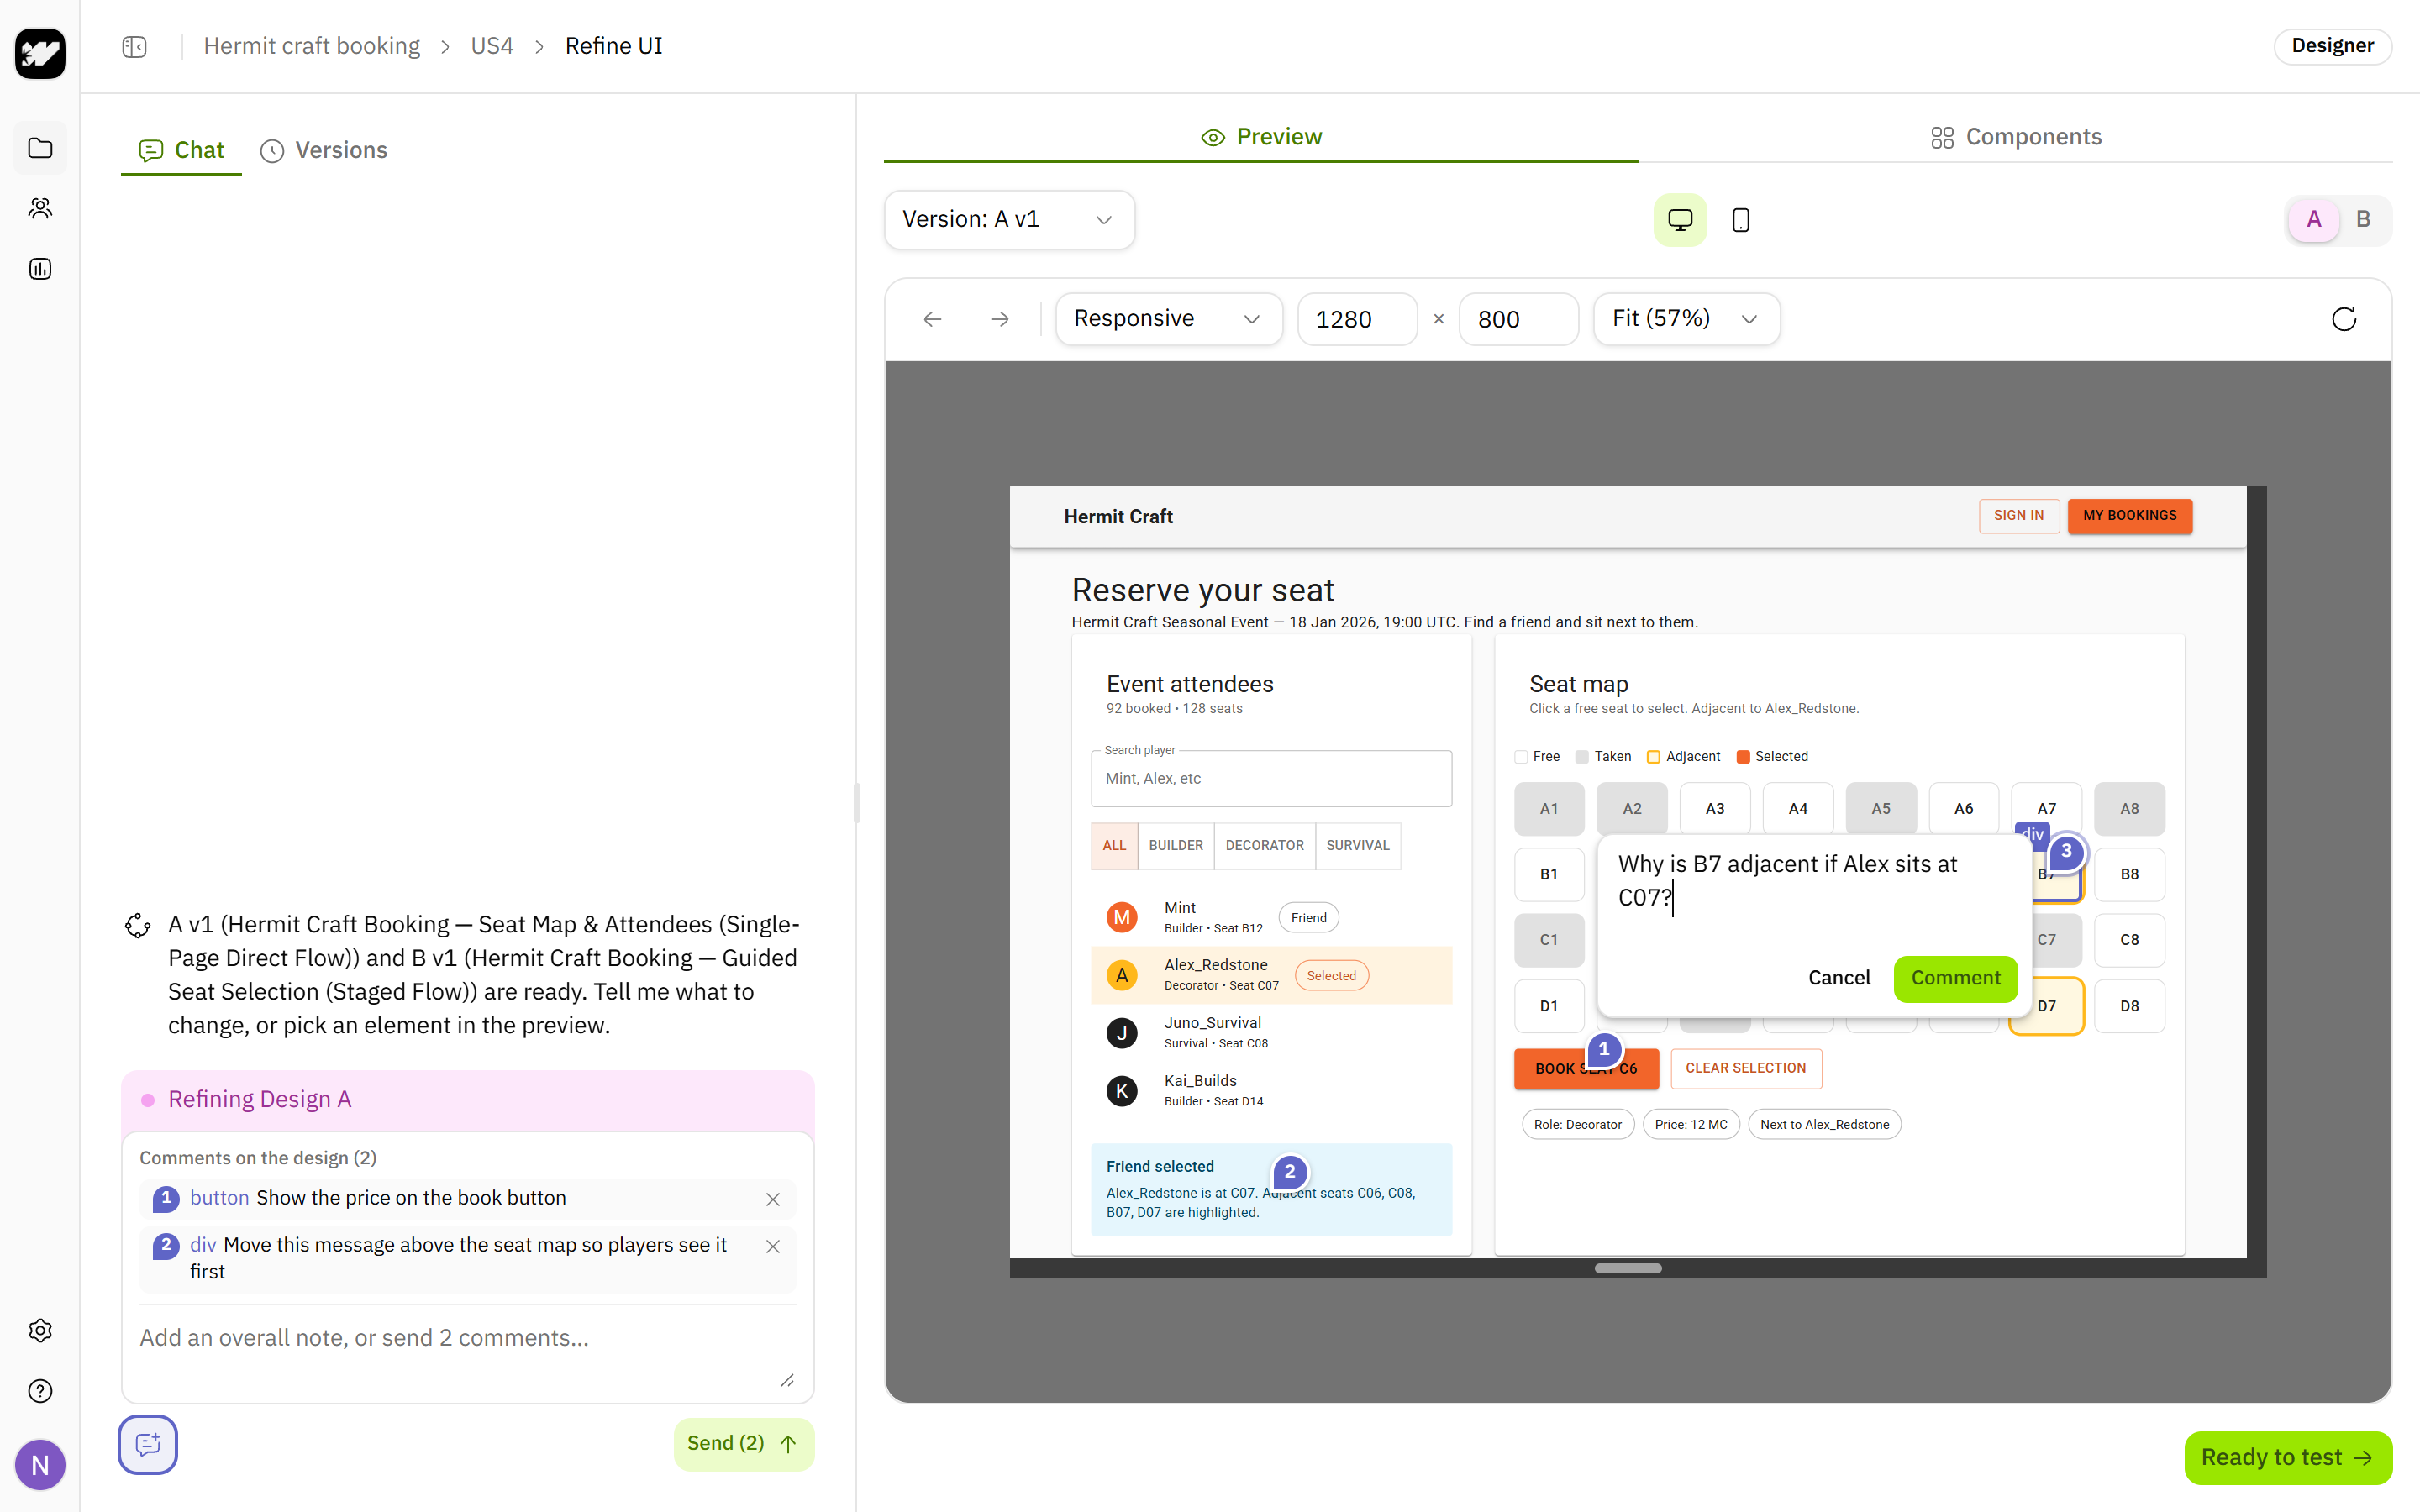
\includegraphics[width=0.9\linewidth]{figures/ch3-methodology/screens/refine-pins.png}
  \caption{หมุดความคิดเห็นบนหน้าตัวอย่างของ variant ในหน้า refine}
  \label{fig:screen-refine-pins}
\end{figure}

\subsection{การพัฒนาหน้าจอเว็บไซต์ของ Usability Tester และผู้มีส่วนได้ส่วนเสีย}
\thaijustify{
  หน้าจอเซสชันการทดสอบ (\texttt{.../sessions}) และรายงาน (\texttt{.../reports}) ปัจจุบันเป็นแท็บในหน้าโปรเจกต์ที่รอเชื่อมกับ API ซึ่ง backend พัฒนาไว้แล้ว (ตารางที่~\ref{tab:api-groups}) หน้าจอของผู้เข้าร่วมทดสอบ และมุมมองของ Client, Developer และ Project Manager อยู่ในแผนของภาคการศึกษาที่ 2
}

